\documentclass[aps,prd,onecolumn,11pt,nofootinbib,superscriptaddress,floatfix]{revtex4-2}

\usepackage{amsmath,amssymb}
\usepackage{graphicx}
\usepackage{booktabs}
\usepackage{array}
\usepackage{xcolor}
\usepackage[colorlinks=true,linkcolor=blue!50!black,citecolor=blue!50!black,urlcolor=blue!50!black]{hyperref}

\graphicspath{{../figures/}}
% Generated by scripts/make_tables.py from results/summary/. Do not edit.
\newcommand{\numdHRKfourLast}{$1.6\times10^{-8}$}
\newcommand{\numdHDOPLast}{$2.5\times10^{-7}$}
\newcommand{\numdHGLtwo}{$5.0\times10^{-12}$}
\newcommand{\numdHGLthreeLast}{$6.7\times10^{-16}$}
\newcommand{\numexpGLthree}{0.48}
\newcommand{\numphaseDOPend}{$1.5\times10^{-3}$}
\newcommand{\numphaseGLthreeEnd}{$7.3\times10^{-11}$}
\newcommand{\numcrossRKfour}{3364}
\newcommand{\numshortDOP}{$776$}
\newcommand{\numshortGLthree}{$5.4\times10^{3}$}
\newcommand{\numlongDOPfour}{$706$}
\newcommand{\numlongGLthreeFour}{$2.1\times10^{3}$}
\newcommand{\numlongGLthreeEight}{$6.2\times10^{3}$}
\newcommand{\numpsDOPdecade}{0.33}
\newcommand{\numpsRKfourDecade}{1.45}
\newcommand{\numpsGLthreeDecade}{2.26}
\newcommand{\numpsGLthreeSaturation}{6.0}
\newcommand{\numpsPlainRKfour}{14.5}
\newcommand{\numpsCompRKfour}{5.0}
\newcommand{\numiscoDPfive}{-0.252}
\newcommand{\numiscoGLtwo}{1.09}
\newcommand{\numiscoGLthree}{1.53}
\newcommand{\numcircPlain}{$5.5\times10^{-6}$}
\newcommand{\numcircComp}{$5.1\times10^{-11}$}
\newcommand{\numcircPlainExp}{2.05}


% Notation
\newcommand{\dd}{\mathrm{d}}
\newcommand{\order}{\mathcal{O}}
\newcommand{\fig}[1]{Fig.~\ref{fig:#1}}
\newcommand{\tab}[1]{Table~\ref{tab:#1}}
\newcommand{\RQ}[1]{RQ#1}
\newcommand{\repo}{\url{https://github.com/NugiePhysics/geodesic-integrators}}

\begin{document}

\title{Geometric versus classical integrators for Schwarzschild geodesics:\\
error growth, invariants and cost over short and long integrations}

\author{Nugie Saputra}
\email{nugi.physics@gmail.com}

\date{October 2026}

\begin{abstract}
Numerical geodesics underlie black-hole imaging and the modelling of extreme-mass-ratio
inspirals, yet the choice of integrator is often made by habit. We compare eight integrators
on timelike and null geodesics of the Schwarzschild metric: the classical Runge--Kutta method
(RK4), the embedded pairs DP5(4) and DOP853, the Gauss--Legendre collocation methods of order
2, 4 and 6, and Tao's explicit symplectic scheme of order 2 and 4. Each is applied to the
second-order geodesic equation and to Hamilton's equations, and every error is measured
against a closed-form reference built from elliptic integrals and functions. Over $10^4$
radial periods the Runge--Kutta methods drift linearly in the mass shell and quadratically in
phase, while the symplectic methods keep the mass-shell error bounded and the phase error
linear; sixth-order Gauss--Legendre reaches round-off and then follows Brouwer's
$N^{1/2}$ law. Gauss--Legendre applied to the second-order system, where it is symmetric but
not symplectic, conserves as well as in canonical variables. For short integrations DOP853 is
the cheapest method at every accuracy; over 1000 periods only sixth-order Gauss--Legendre
reaches a phase error of $10^{-8}$. On the photon sphere every method survives at most about
six orbits, gaining $\ln 10/2\pi$ orbits per decade of accuracy as predicted, and plain
floating-point summation fakes a longer survival. At the ISCO the time to plunge grows
algebraically, as $\varepsilon^{-1/4}$ in the size of the integration error, and the sign of
the error decides whether the orbit plunges at all. Every figure and table is regenerated from
a clean checkout by one command.
\end{abstract}

\maketitle

\section{Introduction}
\label{sec:introduction}

Geodesics of black-hole spacetimes are integrated numerically in two very different regimes.
Ray tracing for images of accretion flows, such as those behind the Event Horizon Telescope
results~\cite{eht2019}, follows millions of photons for a short affine time each; codes such
as GRay~\cite{chan2013}, geokerr~\cite{dexter2009}, RAPTOR~\cite{bronzwaer2018} and
GYOTO~\cite{vincent2011} are built around adaptive Runge--Kutta methods or semi-analytic
solutions. The evolution of bound orbits, as in the adiabatic modelling of
extreme-mass-ratio inspirals, follows a few orbits for $10^3$--$10^5$ revolutions, where the
long-time behaviour of the integration error matters more than its size after one step.
Geometric integrators~\cite{gni2006} are designed for the second regime, and several have been
adapted to geodesics: Gauss collocation with a symmetric step-size control~\cite{seyrich2012},
explicit symplectic splittings for Schwarzschild~\cite{wang2021}, and Tao's extended phase
space~\cite{tao2016,pihajoki2015}, which the FANTASY code applies to arbitrary
metrics~\cite{christian2021}.

Comparisons between these families are usually made on one test problem, one formulation and
one length of integration. This report compares them systematically, on the simplest
spacetime where every relevant quantity has a closed form. We ask five research questions:

\begin{description}
\item[\RQ{1}] How do the mass-shell error and the phase error grow over long integrations?
\item[\RQ{2}] Does the formulation, the second-order geodesic equation or Hamilton's
  equations, change which quantities are conserved, and is a symmetric method that is not
  symplectic in the chosen variables enough?
\item[\RQ{3}] Which method reaches a given accuracy at the lowest cost, and how does the answer
  depend on the length of the integration?
\item[\RQ{4}] How far can an integrator extend the life of an orbit on the unstable photon
  sphere, and of an orbit at the marginally stable ISCO?
\item[\RQ{5}] Which integrator should one use for ray tracing, and which for long orbit
  evolution?
\end{description}

The study has four design choices that the results depend on. First, both formulations keep
the full eight-dimensional phase space, so that the conservation of the energy $E$ and the
axial angular momentum $L_z$ can be tested rather than imposed. Second, the integrators see
only a vector field, so the same code runs on toy problems, on Schwarzschild and, later, on
Kerr. Third, the cost of a run is the number of vector-field evaluations, counting every
fixed-point iteration of the implicit methods. Fourth, errors are measured on physical
quantities against exact references: the deflection angle at the radius where the
integration stops, the angle swept per radial period and the orbit $r(\phi)$ through elliptic
functions, and the exit time from the photon sphere through an elliptic integral.

Section~\ref{sec:formulations} sets out the two formulations and their invariants,
Sec.~\ref{sec:integrators} the integrators and Sec.~\ref{sec:testcases} the test problems and
references. Section~\ref{sec:results} presents the results, ordered by research question.
Section~\ref{sec:discussion} turns them into recommendations, and Sec.~\ref{sec:conclusions}
concludes.

\section{Two formulations of the geodesic problem}
\label{sec:formulations}

We use the signature $(-,+,+,+)$, units $G = c = M = 1$ and Schwarzschild coordinates
$x^\mu = (t, r, \theta, \phi)$ with $f(r) = 1 - 2/r$. A dot is the derivative with respect to
the affine parameter $\lambda$, and $\epsilon = 1$ for timelike geodesics ($\lambda = \tau$),
$\epsilon = 0$ for null ones (normalized by $E = 1$, so that $L = b$).

\paragraph{(a) Second order.} With $u^\mu = \dot x^\mu$ the geodesic equation becomes
\begin{equation}
  \dot x^\mu = u^\mu, \qquad \dot u^\mu = -\Gamma^\mu_{\alpha\beta}(x)\,u^\alpha u^\beta,
  \qquad g_{\mu\nu}u^\mu u^\nu = -\epsilon ,
  \label{eq:second-order}
\end{equation}
a system for $y = (x^\mu, u^\mu) \in \mathbb{R}^8$. The nine independent Christoffel symbols
are listed in Appendix~\ref{app:christoffel}.

\paragraph{(b) Hamiltonian.} The Legendre transform of the Lagrangian
$\mathcal{L} = \tfrac12 g_{\mu\nu}\dot x^\mu \dot x^\nu$, with momenta
$p_\mu = g_{\mu\nu}\dot x^\nu$, gives the super-Hamiltonian~\cite{mtw1973}
\begin{equation}
  H = \tfrac12 g^{\mu\nu}(x)\,p_\mu p_\nu
    = \frac12\left[-\frac{p_t^2}{f} + f p_r^2 + \frac{p_\theta^2}{r^2}
      + \frac{p_\phi^2}{r^2\sin^2\theta}\right],
  \qquad H = -\frac{\epsilon}{2},
  \label{eq:hamiltonian}
\end{equation}
with $\dot x^\mu = g^{\mu\nu}p_\nu$ and $\dot p_\mu = -\tfrac12\partial_\mu
g^{\alpha\beta}p_\alpha p_\beta$, for $y = (x^\mu, p_\mu)$. Only $g^{\mu\nu}$ and its first
derivatives enter, so (b) needs no Christoffel symbols. $H$ is not separable: the kinetic term
depends on position, which rules out the explicit leapfrog family.

\paragraph{Invariants.} Both systems conserve the energy, the axial and total angular momentum
and the mass shell:
\begin{equation}
  E = f u^t = -p_t, \qquad L_z = r^2\sin^2\theta\,u^\phi = p_\phi, \qquad
  L^2 = r^4\left[(u^\theta)^2 + \sin^2\theta(u^\phi)^2\right]
      = p_\theta^2 + \frac{p_\phi^2}{\sin^2\theta}.
  \label{eq:invariants}
\end{equation}
In (b), $t$ and $\phi$ are cyclic, so $\dot p_t$ and $\dot p_\phi$ are the floating-point
number zero. Every Runge--Kutta method, explicit or implicit, then conserves $E$ and $L_z$ bit
for bit, whatever its order, step size or number of iterations. This is a property of the
variables, not a merit of the method. Informative tests of $E$ and $L_z$ are therefore made in
(a), where they are nonlinear functions of the state; in (b) the informative invariants are
$H$ and, for inclined orbits, $L^2$, the Schwarzschild limit of Carter's constant
($Q = L^2 - L_z^2$). None of the invariants is quadratic in the state, so the exact
conservation of quadratic invariants by Gauss methods does not apply; symplectic methods can
only keep their errors bounded~\cite{gni2006}. We report relative errors $\delta H =
|H + \tfrac12|/\tfrac12$ (timelike), $|H|/E^2$ (null), and $\delta E = |E - E_0|/E_0$, and
likewise for $L_z$ and $L^2$.

\paragraph{Symplecticity and reversibility.} Formulation (b) is canonical; a symplectic method
applied to it produces symplectic maps, and backward error analysis bounds the energy error
over exponentially long times~\cite{gni2006}. Formulation (a) describes the same flow in the
non-canonical variables $(x, u)$, where the symplectic form has $x$-dependent coefficients; a
Gauss method applied to (a) is symmetric but not symplectic. Both systems are reversible with
respect to $\rho(x, v) = (x, -v)$, and for integrable reversible systems symmetric methods
share the long-time behaviour of symplectic ones~\cite[Ch.~XI]{gni2006}. Comparing
Gauss--Legendre in (a) and (b) tests whether reversibility alone suffices here (\RQ{2}).

\paragraph{Initial data.} The constraint is a quadratic in one momentum component, solved in
a cancellation-free form with the sign of the velocity. Near a radial turning point
$p_r = \pm\sqrt{E^2 - V_\mathrm{eff}}/f$ is computed from a difference of nearly equal numbers
and comes out of order $\sqrt{\epsilon_\mathrm{mach}}$ instead of zero. Bound and circular
orbits therefore start exactly at a turning point, with $p_r = 0$ and the constraint solved
for $p_t$. The initial relative constraint is at most $3.3\times10^{-16}$ on every orbit of
the study, in both formulations.

\section{Integrators}
\label{sec:integrators}

All integrators share one interface: they receive the vector field $F(y)$ (and, for Tao's
method, the canonical structure of the state) and know nothing about the metric. The
properties of the eight methods are collected in \tab{methods}.

\begin{table*}[t]
\caption{\label{tab:methods}The integrators (T1). For the implicit methods the cost per step
is the number of stages times the number of fixed-point iterations; the measured values are
averages over $10^4$ periods of the orbit $(p, e) = (20, 0.5)$ at 1000 steps per period.}
\centering\small
\resizebox{\textwidth}{!}{% Generated by scripts/make_tables.py from results/summary/. Do not edit.
\begin{tabular}{llcccclc}
\toprule
Method & Structure & Order & Sympl. & Symm. & Adapt. & Evaluations per step & Form. \\
\midrule
RK4 & explicit Runge-Kutta & 4 & no & no & no & 4 & (a), (b) \\
DP5 & explicit embedded pair 5(4) & 5 & no & no & yes & 6 & (a), (b) \\
DOP853 & explicit embedded pair 8(5,3) & 8 & no & no & yes & 12 & (a), (b) \\
GL1 & implicit midpoint (Gauss, s = 1) & 2 & yes & yes & no & 1 per iteration; measured 6.8 (b), 7.9 (a) & (a), (b) \\
GL2 & Gauss collocation, s = 2 & 4 & yes & yes & no & 2 per iteration; measured 11.2 (b), 13.0 (a) & (a), (b) \\
GL3 & Gauss collocation, s = 3 & 6 & yes & yes & no & 3 per iteration; measured 14.2 (b), 18.4 (a) & (a), (b) \\
Tao2 & extended phase space, Strang & 2 & yes & yes & no & 3 & (b) only \\
Tao4 & extended phase space, triple jump & 4 & yes & yes & no & 9 & (b) only \\
\bottomrule
\end{tabular}
}
\end{table*}

\paragraph{Explicit Runge--Kutta.} RK4 is the classical four-stage method with a fixed step;
the parameter after $n$ steps is $\lambda_0 + nh$, never a running sum. DP5(4)~\cite{dormand1980}
and DOP853~\cite{hnw1993} are the embedded pairs of SciPy's \texttt{RK45} and \texttt{DOP853},
reimplemented in compiled code with SciPy's step-size controller copied line by line. From a
generic starting point both take the same steps as SciPy and use the same number of
evaluations at tolerances $10^{-4}$--$10^{-12}$; step sizes agree to $10^{-7}$. Events
(periapsis passages, crossings of a radius) are located by root finding on partial steps of
the method itself, so their accuracy matches the order of the method; linear interpolation
would cap the measured order at two.

\paragraph{Gauss--Legendre.} The $s$-stage Gauss methods GL1 (implicit midpoint), GL2 and GL3
have order $2s$, and are symplectic and symmetric~\cite{gni2006}. The stage equations are
solved by fixed-point iteration on the increments $Z_i = Y_i - y_n$, started from the
collocation polynomial of the previous step. The iteration runs until the norm of the
correction stops decreasing, the rule recommended for round-off-limited
integrations~\cite{hairer2008}, with a guard: stagnation counts only once the correction is
within 100 ulp of the increments, because on rotation-like problems the correction can wobble
long before round-off. The update $y_{n+1} = y_n + d^\mathsf{T}Z$, $d = b^\mathsf{T}A^{-1}$, is
added with compensated summation~\cite{kahan1965}. An optional absolute tolerance on the
correction replaces the stagnation rule for the experiment of Sec.~\ref{sec:method-details}.

\paragraph{Tao's method.} Tao~\cite{tao2016} integrates two copies $(q, p)$ and $(x, y)$ of the
state with
\begin{equation}
  \tilde H(q, p, x, y) = H(q, y) + H(x, p) + \frac{\omega}{2}\left(|q - x|^2 + |p - y|^2\right).
  \label{eq:tao}
\end{equation}
The flows of the first two terms are explicit shifts, the third rotates $(q - x, p - y)$ by the
angle $2\omega\delta$. The second-order method is the Strang composition
$\phi_A^{h/2}\phi_B^{h/2}\phi_C^{h}\phi_B^{h/2}\phi_A^{h/2}$, the fourth-order one its triple
jump with $\gamma_1 = 1/(2 - 2^{1/3})$, $\gamma_2 = 1 - 2\gamma_1$~\cite{yoshida1990}. Each flow
is one call of the vector field of (b); caching the gradient between consecutive flows gives 3
and 9 evaluations per step. Two choices are not fixed by the method. We couple only the
non-cyclic coordinates $(r, \theta)$: coupling $t$ and $\phi$ as well lets the time copies
drift apart by up to $10^4$, and the rotation then feeds that difference into $p_t$, so $E$ is
no longer conserved. And $\omega$ must be chosen; Sec.~\ref{sec:method-details} fixes
$\omega = 10^{-3}$ for all experiments.

\paragraph{Cost.} The cost of a run is its number of vector-field evaluations $n_\mathrm{fev}$,
including every fixed-point iteration and, for Tao, every gradient. Wall times are compared
only between our own compiled implementations, with one thread per process, after
compilation, as the median of repeats; they track $n_\mathrm{fev}$ up to a factor of order
one. One evaluation costs $0.7$--$1.6\,\mu$s inside the drivers on the machine of
Appendix~\ref{app:environment}.

\paragraph{Verification.} Before any geodesic run the integrators were tested on the harmonic
oscillator, the Kepler problem and Tao's nonseparable example $H = \tfrac12(q^2 + 1)(p^2 + 1)$.
The measured orders are $2.00$, $4.00$, $6.00$ for GL1--GL3, $2.00$ and $3.98$ for Tao2 and
Tao4, and $4.05$ for RK4. The one-step maps of GL and Tao preserve the symplectic form to
$2\times10^{-12}$ (the accuracy of the finite-difference Jacobian; Tao in its extended space),
against $4\times10^{-3}$ for RK4, and they are symmetric, $\Psi_{-h}\circ\Psi_h = \mathrm{id}$,
to $2\times10^{-16}$. Over $10^6$ steps of Tao's example their energy error is bounded, while
RK4's doubles from the first to the second half of the run.

\section{Test problems and exact references}
\label{sec:testcases}

\fig{hero} shows the geodesics of the study. Each test case fixes the initial data, the span
of the integration, the events that stop it, an exact reference and an error defined on a
physical quantity, never on the raw state, because the states of (a) and (b) differ.

\begin{figure}[t]
\centering
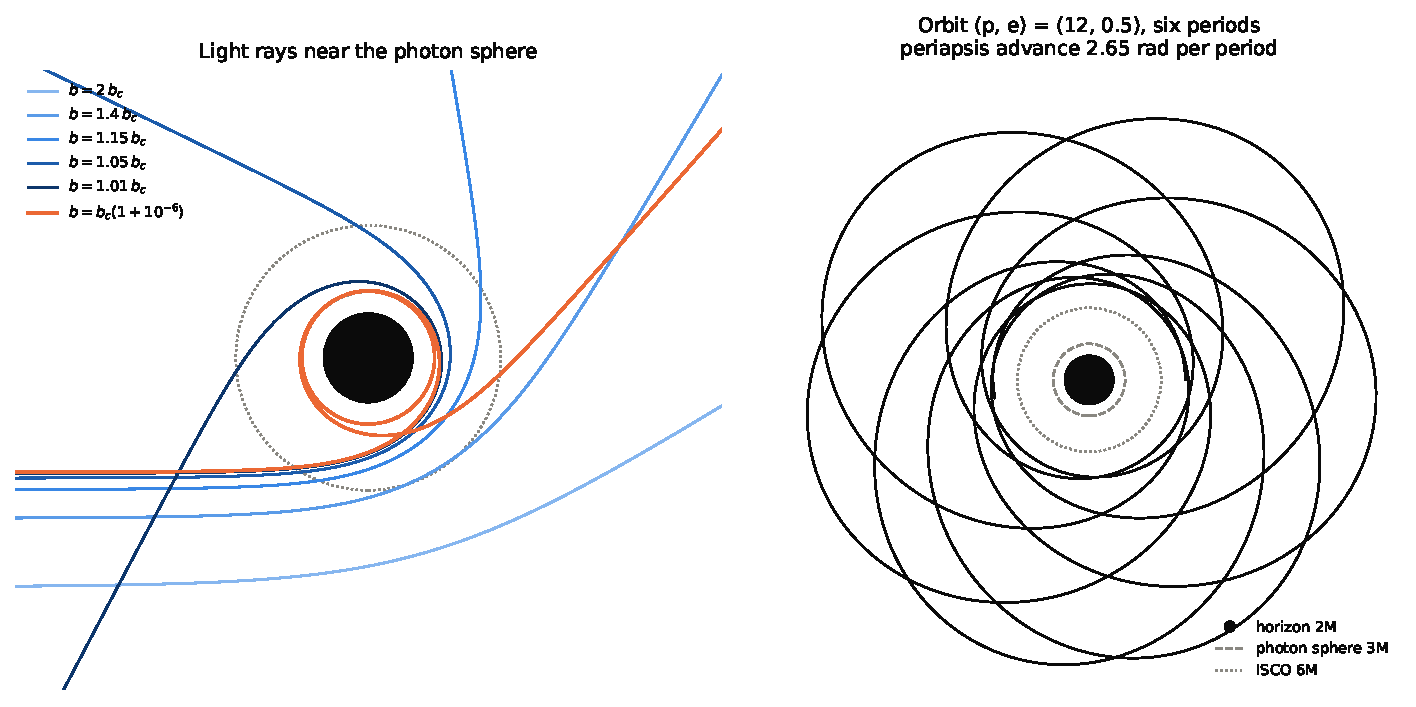
\includegraphics[width=\textwidth]{F01_hero.pdf}
\caption{\label{fig:hero}The geodesics of the study in the equatorial plane, with the horizon
($r = 2$), the photon sphere ($r = 3$) and the ISCO ($r = 6$). Left: a parallel bundle of light
rays with impact parameters from $2b_c$ to $b_c(1 + 10^{-6})$; the last winds about twice
around the photon sphere. Right: six radial periods of the bound orbit $(p, e) = (12, 0.5)$.}
\end{figure}

\paragraph{TC1, light deflection.} A photon with impact parameter $b > b_c = 3\sqrt3$ starts at
$r_\mathrm{far}$ and is followed to $r_\mathrm{far}$ again. With $u = 1/r$ and the roots
$u_1 < 0 < u_2 < u_3$ of $2u^3 - u^2 + b^{-2}$, the angle swept is
\begin{equation}
  \Delta\phi(r_\mathrm{far}) = \frac{4F(\psi\,|\,m)}{\sqrt{2(u_3 - u_1)}}, \qquad
  m = \frac{u_2 - u_1}{u_3 - u_1}, \qquad
  \sin^2\psi = \frac{(u_3 - u_1)(u_2 - u_\mathrm{far})}{(u_2 - u_1)(u_3 - u_\mathrm{far})},
  \label{eq:deflection}
\end{equation}
which for $r_\mathrm{far} \to \infty$ is Darwin's result~\cite{darwin1959,iyer2007}. The
reference uses the same $r_\mathrm{far}$ as the integration: comparing with the asymptotic
angle would leave a systematic error of order $b/r_\mathrm{far}^2$. Equation
(\ref{eq:deflection}), Darwin's form in terms of the periapsis and a direct 30-digit quadrature
agree to double precision for $b \in [5.2, 10^4]$. TC1b takes $b = b_c(1 + 10^{-k})$,
$k = 1, \dots, 10$, where the number of windings grows like $-\ln(b/b_c - 1)/2\pi$
(Bozza's strong-deflection limit~\cite{bozza2002}).

\paragraph{TC2, photon sphere.} A photon starts at a turning point $r_0 = 3 + \delta_0$ with
$b = b_c$ and is followed until $|r - 3| > 0.1$. Small offsets grow like
$\cosh(\lambda_L t)$ with $\lambda_L = 1/(3\sqrt3)$~\cite{cardoso2009}, a factor $e^{2\pi}
\approx 535$ per orbit; the exact exit angle is an elliptic integral from the turning point.
The equatorial orbit with $\delta_0 = 0$ is an exact fixed point of every Runge--Kutta map:
the radial components of the vector field vanish and $t$, $\phi$ are linear in $\lambda$. It
survived 900 orbits in a first test. The experiments therefore tilt the orbital plane by
$45^\circ$, so that truncation errors in $L^2$ reach $r$.

\paragraph{TC3, circular orbits.} Timelike circular orbits with $E = f/\sqrt{1 - 3/r_c}$,
$L = \sqrt{r_c/(1 - 3/r_c)}$ and $\Omega = r_c^{-3/2}$. Like the photon sphere they are fixed
points of the radial dynamics; their errors measure round-off, not truncation. TC3m starts on
the ISCO ($r = 6$, $E = \sqrt{8/9}$, $L = 2\sqrt3$) in a plane inclined by $45^\circ$ and stops
when $|r - 6| > 1$.

\paragraph{TC4 and TC5, eccentric orbits.} Bound orbits are labelled by the semi-latus rectum
$p$ and eccentricity $e$~\cite{cutler1994}, with $r_p = p/(1 + e)$ and $r_a = p/(1 - e)$. The
orbit equation $(\dd u/\dd\phi)^2 = 2(u - u_1)(u - u_2)(u - u_3)$ has $u_1 = (1 - e)/p$,
$u_2 = (1 + e)/p$ and $u_3 = \tfrac12 - 2/p$, which gives the angle per radial period and the
orbit in closed form~\cite{chandrasekhar1983}:
\begin{equation}
  \Phi = \frac{4K(m)}{\sqrt{2(u_3 - u_1)}}, \qquad
  u(\phi) = u_1 + (u_2 - u_1)\,\mathrm{cd}^2\!\left(\sqrt{\tfrac{u_3 - u_1}{2}}\,\phi\;\middle|\;m\right),
  \qquad m = \frac{u_2 - u_1}{u_3 - u_1}.
  \label{eq:orbit}
\end{equation}
The radial periods in proper and coordinate time come from a 30-digit quadrature in the angle
$\chi$ of $r = \tfrac12(r_a + r_p) - \tfrac12(r_a - r_p)\cos\chi$, which removes both
turning-point singularities and gives $\Phi$ a second time (agreement $10^{-16}$). The
long-term case TC5 follows $(20, 0.5)$ for $10^3$--$10^4$ periods; its phase error is
$\phi_N - N\Phi$ at the $N$-th periapsis, which needs no reference integration.

\paragraph{TC6, inclined orbits.} The orbit $(20, 0.5)$ in planes inclined by $30^\circ$,
$60^\circ$ and $85^\circ$. The references are $L^2$ and the orientation of the orbital plane,
measured by the angle between the angular-momentum vector $(L_x, L_y, L_z)$ at each sample and
at the start.

\paragraph{Validation.} \tab{validation} compares tightly integrated values (DOP853, tolerance
$10^{-13}$, formulation (b)) with every reference. All agree to $10^{-11}$ or better, except
the cases amplified by the photon sphere, which agree to about $10^{-8}$.

\begin{table*}[t]
\caption{\label{tab:validation}Validation (T2): DOP853 at tolerance $10^{-13}$ in formulation
(b) against the exact references. The last row compares with the value listed by the
predecessor project, \texttt{schwarzschild-geodesics}: its ``analytic'' 2.127093985 was
evaluated at the smallest sampled radius rather than the true periapsis. The exact value,
from the closed form and a 40-digit quadrature, is 2.12709400813.}
\centering\footnotesize
% Generated by scripts/make_tables.py from results/summary/. Do not edit.
\begin{tabular}{lrrr}
\toprule
Check & Numerical & Analytical & Difference \\
\midrule
TC1 deflection $\Delta$$\phi$(r\_far), b = 6, r\_far = 1000 & 4.84898 & 4.84898 & $6.1\times10^{-13}$ \\
TC1 deflection $\Delta$$\phi$(r\_far), b = 40, r\_far = 10000 & 3.2417 & 3.2417 & $4.1\times10^{-13}$ \\
TC1 deflection $\Delta$$\phi$(r\_far), b = 1000, r\_far = 10000 & 2.94527 & 2.94527 & $3.5\times10^{-14}$ \\
TC1b windings, b = b\_c(1 + 1e-6) & 2.63346 & 2.63346 & $1.1\times10^{-8}$ \\
TC2 orbits before $|$r - 3$|$ $>$ 0.1, r0 = 3 + 1e-6 & 1.93916 & 1.93916 & $1.2\times10^{-8}$ \\
TC2 growth rate of $|$r - 3$|$ in t (Lyapunov exponent) & 0.192515 & 0.19245 & $6.5\times10^{-5}$ \\
TC3 circular orbit r\_c = 10: d$\phi$/dt & 0.0316228 & 0.0316228 & $0$ \\
TC3 circular orbit r\_c = 6: d$\phi$/dt & 0.0680414 & 0.0680414 & $2.6\times10^{-15}$ \\
TC4 periapsis advance, (p, e) = (20, 0.5) & 1.23386 & 1.23386 & $5.6\times10^{-13}$ \\
TC4 radial period in proper time, (p, e) = (20, 0.5) & 930.547 & 930.547 & $8.0\times10^{-11}$ \\
TC4 periapsis advance, (p, e) = (7.5, 0.5) & 9.35519 & 9.35519 & $1.3\times10^{-11}$ \\
TC4 radial period in proper time, (p, e) = (7.5, 0.5) & 307.14 & 307.14 & $5.0\times10^{-11}$ \\
TC6 inclined 60$^\circ$: in-plane angle after 2 periods & 15.0341 & 15.0341 & $1.6\times10^{-11}$ \\
TC6 inclined 60$^\circ$: tilt of the orbital plane (rad) & 1.58374e-13 & 0 & $1.6\times10^{-13}$ \\
TC6 inclined 60$^\circ$: max relative change of L$^2$ & 1.35381e-13 & 0 & $1.4\times10^{-13}$ \\
Old README: precession r\_apo = 20, L = 4.2 & 2.12709 & 2.12709 & $2.3\times10^{-8}$ \\
\bottomrule
\end{tabular}

\end{table*}

\section{Results}
\label{sec:results}

\subsection{Convergence on geodesics}
\label{sec:convergence}

Every fixed-step method reaches its theoretical order on geodesics, in both formulations
(\fig{convergence}, \tab{orders}). On the strong-field orbit $(7.5, 0.5)$ the measured orders
are within $\pm0.05$ of theory, on the deflection with $b = 6$ within $\pm0.08$. GL1 and Tao2
are almost indistinguishable in (b), and GL1 is about 35 times less accurate in (a) than in (b)
at the same step. The adaptive pairs show tolerance proportionality: the global error falls
like $\mathrm{tol}^{0.85\text{--}1.04}$ for DP5 and DOP853, on the same curves as SciPy's
(\fig{tolerance}). On $(20, 0.5)$ RK4 stays pre-asymptotic over the whole usable range
(slopes 4.5 to 4.07 before round-off), which is why the orders are measured on the
strong-field orbit.

\begin{figure}[t]
\centering
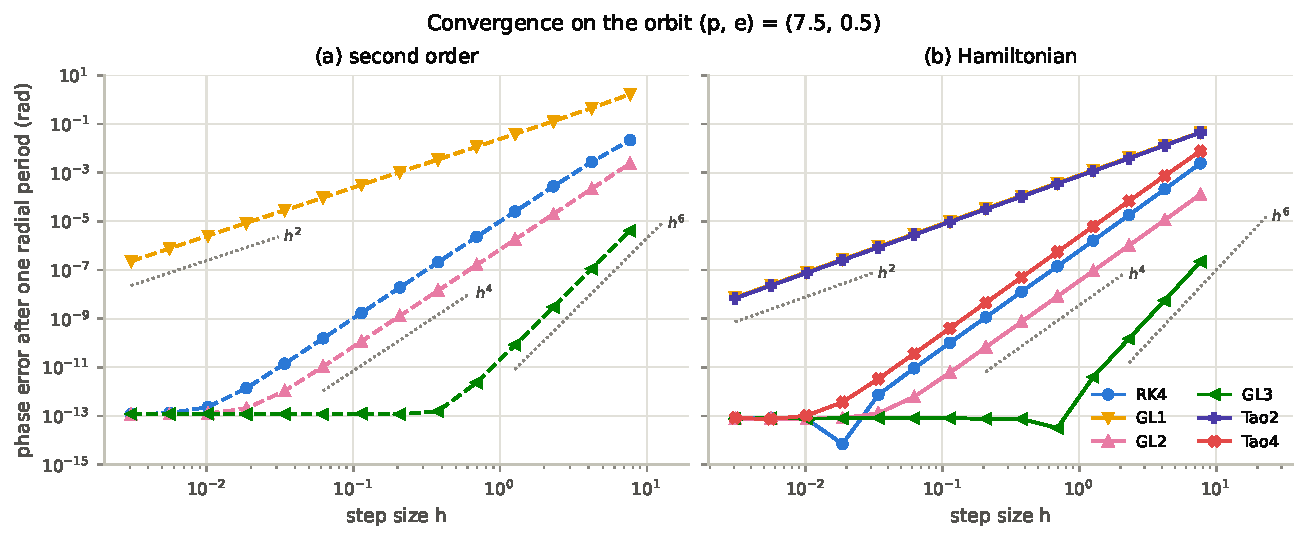
\includegraphics[width=0.95\textwidth]{F04_convergence.pdf}
\caption{\label{fig:convergence}Convergence of the fixed-step methods: error against step size
for the deflection $b = 6$ (error in $\Delta\phi(r_\mathrm{far})$) and one radial period of
the orbit $(7.5, 0.5)$ (error in $\phi$), in both formulations, with reference slopes 2, 4
and 6 (F4).}
\end{figure}

\begin{table}[t]
\caption{\label{tab:orders}Measured order of convergence (T3), least-squares slope over the
asymptotic range with its standard error.}
\centering\small
% Generated by scripts/make_tables.py from results/summary/. Do not edit.
\begin{tabular}{lccccc}
\toprule
Method & Theory & Deflection (a) & Deflection (b) & Orbit (a) & Orbit (b) \\
\midrule
RK4 & 4 & $4.08 \pm 0.02$ & $3.96 \pm 0.01$ & $3.98 \pm 0.01$ & $4.01 \pm 0.00$ \\
GL1 & 2 & $2.00 \pm 0.00$ & $2.00 \pm 0.00$ & $2.00 \pm 0.00$ & $2.00 \pm 0.00$ \\
GL2 & 4 & $4.00 \pm 0.00$ & $3.98 \pm 0.01$ & $3.98 \pm 0.01$ & $4.00 \pm 0.00$ \\
GL3 & 6 & $6.00 \pm 0.00$ & $6.06 \pm 0.04$ & $5.97 \pm 0.01$ & $6.05 \pm 0.01$ \\
Tao2 & 2 & -- & $2.00 \pm 0.00$ & -- & $2.00 \pm 0.00$ \\
Tao4 & 4 & -- & $4.01 \pm 0.00$ & -- & $4.00 \pm 0.00$ \\
\bottomrule
\end{tabular}

\end{table}

\begin{figure}[t]
\centering
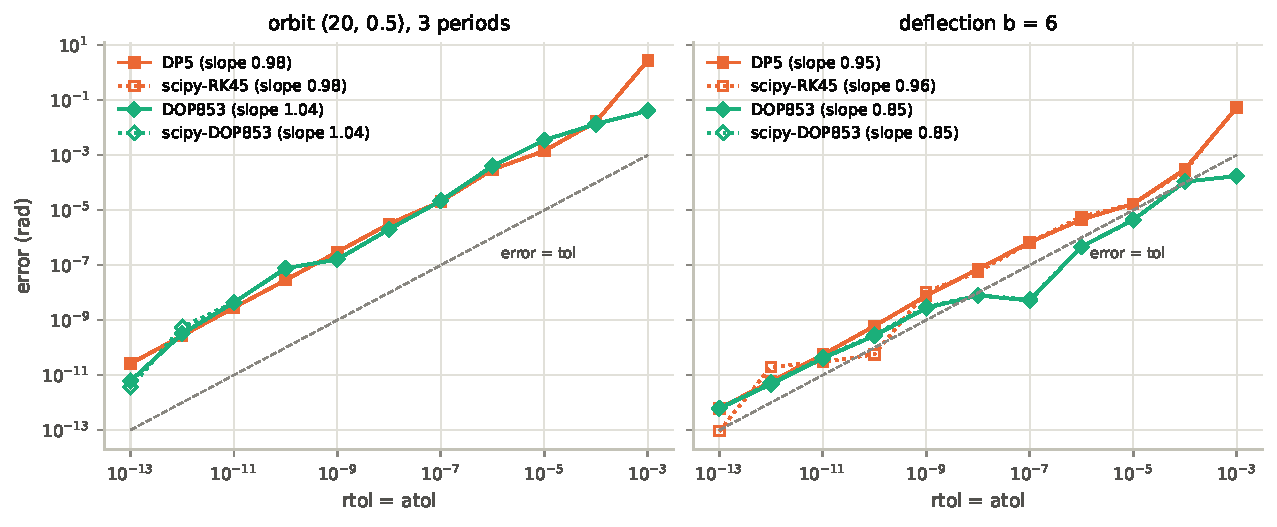
\includegraphics[width=0.6\textwidth]{F05_tolerance.pdf}
\caption{\label{fig:tolerance}Tolerance proportionality of the adaptive pairs: global error
against $\mathrm{rtol} = \mathrm{atol}$, ours and SciPy's (F5).}
\end{figure}

\subsection{Short integrations: cost per accuracy (RQ3)}
\label{sec:short}

\fig{work-precision} and \tab{cost} compare the cost of reaching a given error on three short
problems: the deflection $b = 6$, three periods of $(20, 0.5)$ and two periods of the same
orbit inclined by $60^\circ$. \textbf{DOP853 is the cheapest method on every problem and at
every accuracy.} To reach $10^{-10}$ in formulation (b) it needs $1.4$--$3.2\times10^3$
evaluations, against $1.6$--$3.6\times10^4$ for GL3, the best fixed-step method, and
$3.5\times10^4$--$1.7\times10^5$ for RK4. Tao4 costs 1.2--10 times as much as RK4 for the same
error, and GL1 and Tao2 never reach $10^{-10}$ in the sweep. Formulation (b) is the cheaper
one for most pairs of method and problem, but not all: on the inclined orbit DOP853 and GL3
reach $10^{-10}$ more cheaply in (a).

\begin{figure}[t]
\centering
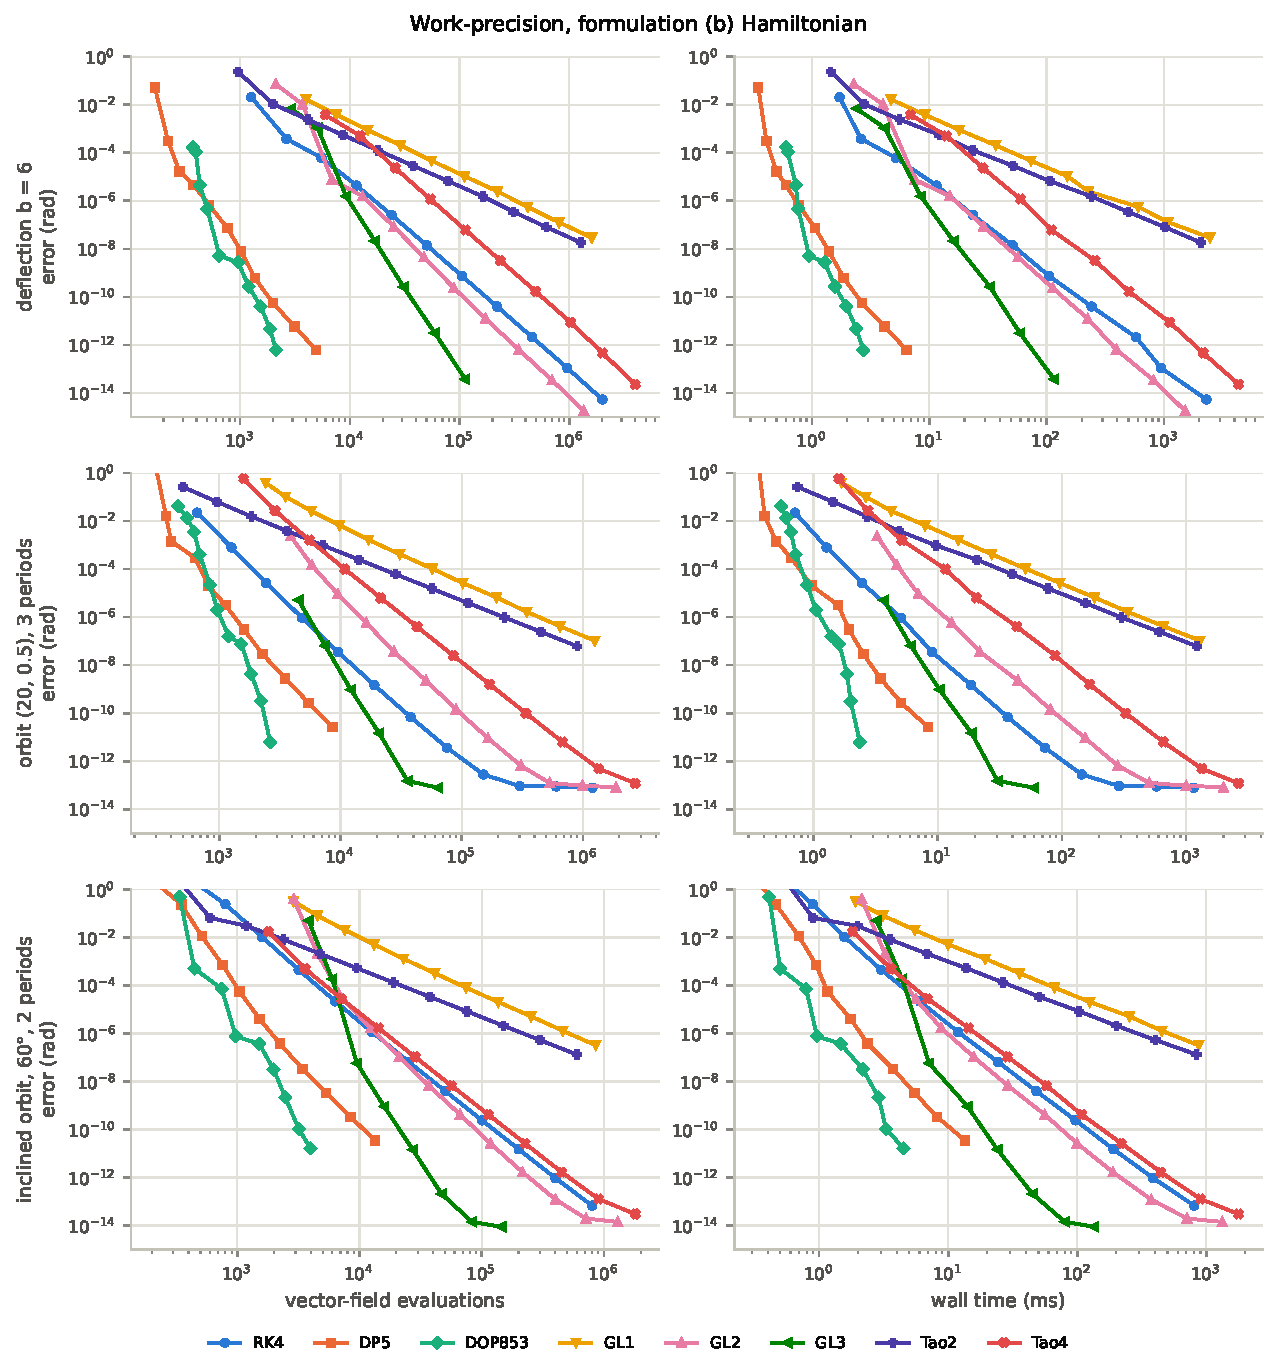
\includegraphics[width=0.9\textwidth]{F06_work_precision_b.pdf}
\caption{\label{fig:work-precision}Work-precision in formulation (b): error against
vector-field evaluations (left) and wall time (right) for the three short problems (F6).
Each curve is the Pareto front of a sweep over 12 step sizes or 11 tolerances.}
\end{figure}

\begin{table*}[t]
\caption{\label{tab:cost}Evaluations needed to reach the error $10^{-6}$ or $10^{-10}$ (T5),
interpolated along each method's work-precision front, in formulation (b) with (a) in
parentheses. A dash means the target was not reached in the sweep.}
\centering\small
\resizebox{\textwidth}{!}{% Generated by scripts/make_tables.py from results/summary/. Do not edit.
\begin{tabular}{lrrrrrr}
\toprule
Method & Deflection, $10^{-6}$ & $10^{-10}$ & Orbit, $10^{-6}$ & $10^{-10}$ & Inclined, $10^{-6}$ & $10^{-10}$ \\
\midrule
RK4 & $1.7\times10^{4}$ ($1.7\times10^{4}$) & $1.7\times10^{5}$ ($1.6\times10^{5}$) & $4.8\times10^{3}$ ($8.3\times10^{3}$) & $3.5\times10^{4}$ ($8.4\times10^{4}$) & $1.3\times10^{4}$ ($1.2\times10^{4}$) & $1.3\times10^{5}$ ($1.3\times10^{5}$) \\
DP5 & $487$ ($1.3\times10^{3}$) & $1.8\times10^{3}$ ($7.1\times10^{3}$) & $1.3\times10^{3}$ ($2.5\times10^{3}$) & $6.6\times10^{3}$ (--) & $1.9\times10^{3}$ ($1.6\times10^{3}$) & $1.1\times10^{4}$ (--) \\
DOP853 & $476$ ($1.2\times10^{3}$) & $1.4\times10^{3}$ (--) & $1.0\times10^{3}$ ($1.5\times10^{3}$) & $2.3\times10^{3}$ ($3.5\times10^{3}$) & $958$ ($1.4\times10^{3}$) & $3.2\times10^{3}$ ($2.4\times10^{3}$) \\
GL1 & $3.3\times10^{5}$ ($1.9\times10^{6}$) & -- & $4.3\times10^{5}$ ($9.6\times10^{5}$) & -- & $5.2\times10^{5}$ ($7.4\times10^{5}$) & -- \\
GL2 & $1.4\times10^{4}$ ($4.9\times10^{4}$) & $1.1\times10^{5}$ ($3.6\times10^{5}$) & $1.5\times10^{4}$ ($2.1\times10^{4}$) & $9.7\times10^{4}$ ($1.4\times10^{5}$) & $1.4\times10^{4}$ ($1.8\times10^{4}$) & $8.9\times10^{4}$ ($1.2\times10^{5}$) \\
GL3 & $9.8\times10^{3}$ ($1.9\times10^{4}$) & $3.6\times10^{4}$ ($6.4\times10^{4}$) & $5.4\times10^{3}$ ($7.5\times10^{3}$) & $1.6\times10^{4}$ ($2.0\times10^{4}$) & $8.1\times10^{3}$ ($8.4\times10^{3}$) & $2.1\times10^{4}$ ($1.8\times10^{4}$) \\
Tao2 & $2.0\times10^{5}$ (--) & -- & $2.2\times10^{5}$ (--) & -- & $2.2\times10^{5}$ (--) & -- \\
Tao4 & $5.6\times10^{4}$ (--) & $5.6\times10^{5}$ (--) & $3.4\times10^{4}$ (--) & $3.4\times10^{5}$ (--) & $1.6\times10^{4}$ (--) & $1.6\times10^{5}$ (--) \\
\bottomrule
\end{tabular}
}
\end{table*}

The deflection angle itself is reproduced to $10^{-14}$ relative far from the hole and to
$10^{-11}$ at $b - b_c = 10^{-3}$, where the problem amplifies errors (\fig{deflection}). The
fourth-order weak-field series is good to $10^{-11}$ at $b \approx 2000$ and off by more than
1\% below $b \approx 10$; Bozza's limit is accurate near $b_c$ and fails above
$b - b_c \approx 1$. Near the critical impact parameter the number of windings follows
$-\ln(b/b_c - 1)/2\pi$, and the integration error grows exactly like the condition number
$1/(b - b_c)$: $3.3\times10^{-13}/(b - b_c)$ windings in (b) and $1.4\times10^{-10}/(b - b_c)$
in (a) (\fig{windings}). The periapsis advance agrees with $\Phi - 2\pi$ to
$4\times10^{-13}$ away from the separatrix and to $1.5\times10^{-8}$ at $p = 7.02$, where the
orbit sweeps 3.4 extra turns per period and the weak-field value $6\pi/p$ is off by 87\%
(\fig{precession}).

\begin{figure}[t]
\centering
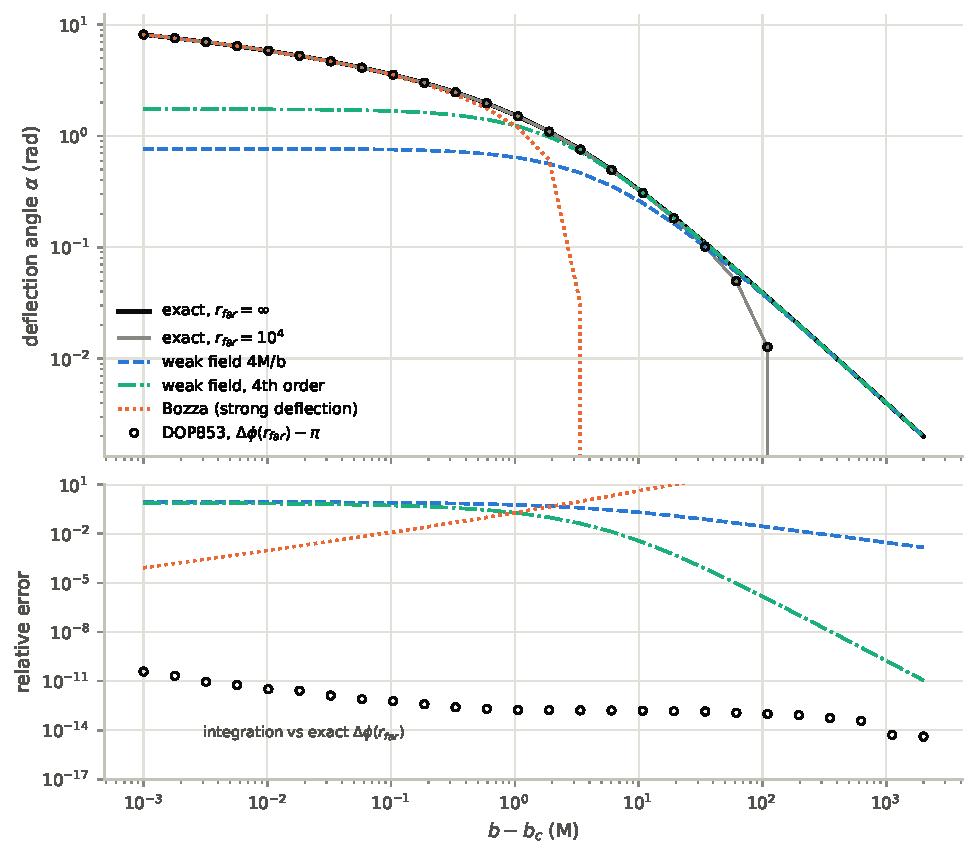
\includegraphics[width=0.6\textwidth]{F02_deflection.pdf}
\caption{\label{fig:deflection}Deflection angle against $b - b_c$: exact, weak-field series,
Bozza's limit and the integration (DOP853, tolerance $10^{-13}$); bottom, relative errors (F2).}
\end{figure}

\begin{figure}[t]
\centering
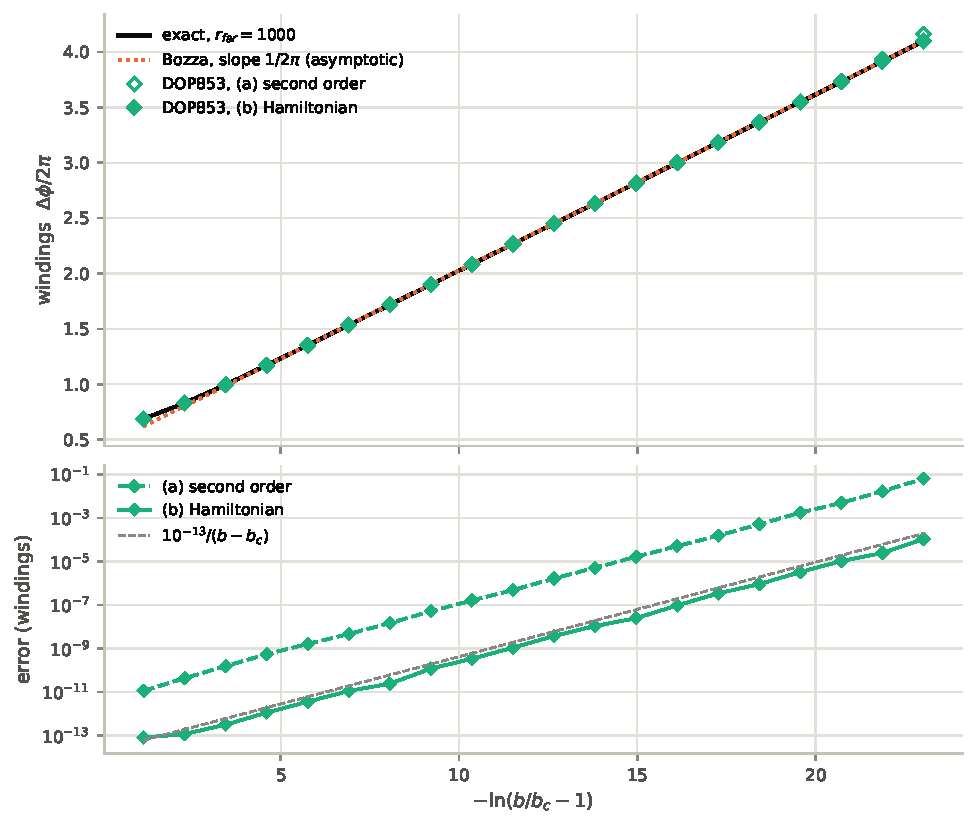
\includegraphics[width=0.48\textwidth]{F12_windings.pdf}\hfill
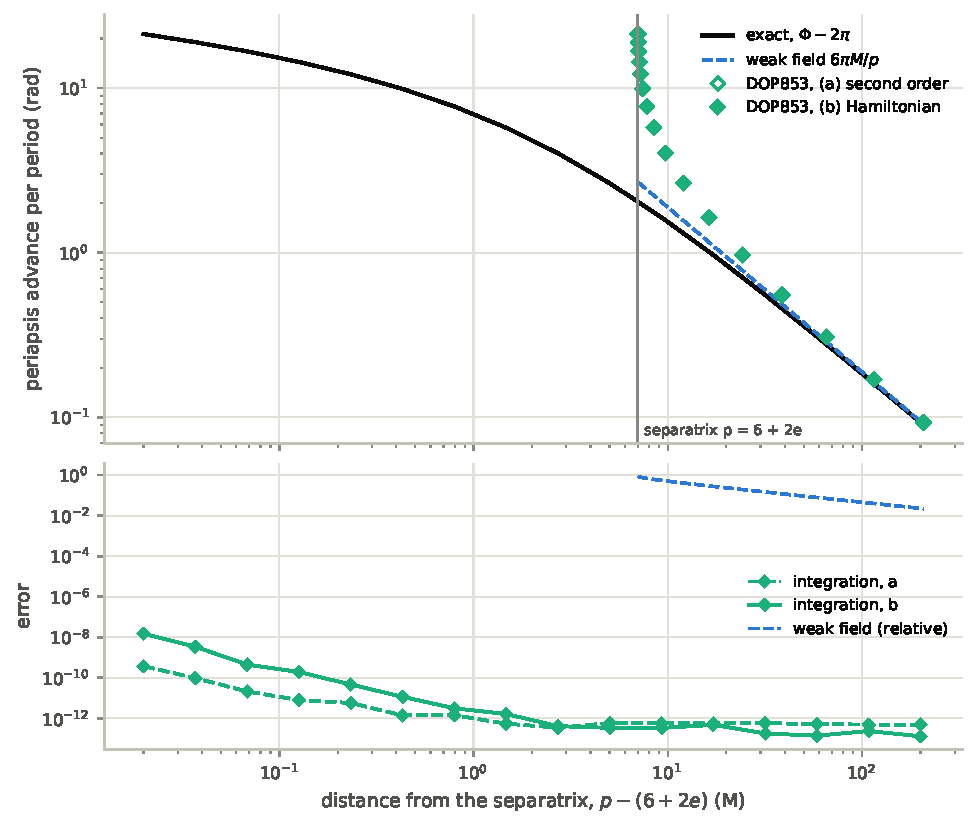
\includegraphics[width=0.48\textwidth]{F13_precession.pdf}
\caption{\label{fig:windings}\label{fig:precession}Left: windings near the critical impact
parameter and their integration error, which follows the condition number $1/(b - b_c)$ (F12).
Right: periapsis advance against $p$, exact, integrated and weak-field (F13).}
\end{figure}

\subsection{Long integrations: growth of the errors (RQ1)}
\label{sec:long}

\fig{energy} shows the mass-shell error over $10^4$ radial periods of $(20, 0.5)$, with 1000
steps per period for the fixed-step methods and tolerance $10^{-10}$ for the adaptive pairs.
The hypothesis of \RQ{1} holds without exception (\tab{growth}). \textbf{RK4, DP5 and DOP853
drift linearly}: the exponents fitted over the last decade are $1.000 \pm 0.002$, and
$|\delta H|$ reaches \numdHRKfourLast{} (RK4) and \numdHDOPLast{} (DOP853).
\textbf{GL1, GL2, Tao2 and Tao4 are bounded}, with exponents below $3\times10^{-3}$; GL2 stays
at \numdHGLtwo{}. GL3's truncation error is below round-off. Its error grows from $10^{-16}$ to
\numdHGLthreeLast{} with exponent \numexpGLthree, Brouwer's random walk~\cite{brouwer1937}.

\begin{figure}[t]
\centering
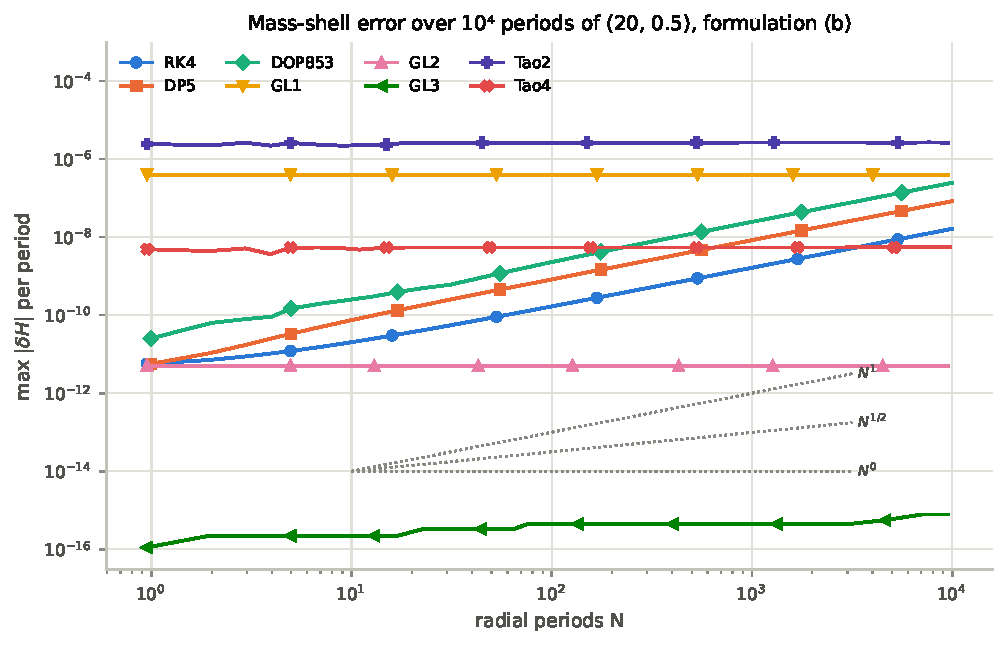
\includegraphics[width=0.7\textwidth]{F07_energy_long_term.pdf}
\caption{\label{fig:energy}Mass-shell error, maximum per radial period, over $10^4$ periods
of $(20, 0.5)$ in formulation (b), drawn as its maximum over logarithmic bins (F7).}
\end{figure}

The phase error at the $N$-th periapsis (\fig{phase}) grows quadratically for the
Runge--Kutta methods (exponents 1.97--2.04) and linearly for GL1, GL2 and Tao ($1.000 \pm
0.001$). A log-log slope is a poor summary of a signed error, so \tab{growth} also fits
$\phi_N - N\Phi = c_1N + c_2N^2$. For RK4 in (b) the constant frequency error $c_1$ and the
drift $c_2$ have opposite signs and cancel near $N = \numcrossRKfour$, the dip in the figure.
GL3's phase error, \numphaseGLthreeEnd{} at $N = 10^4$, is 5 ulp of $\phi \approx
7.3\times10^4$. Its linear growth is the spacing of floating-point numbers growing with
$\phi$.

\begin{figure}[t]
\centering
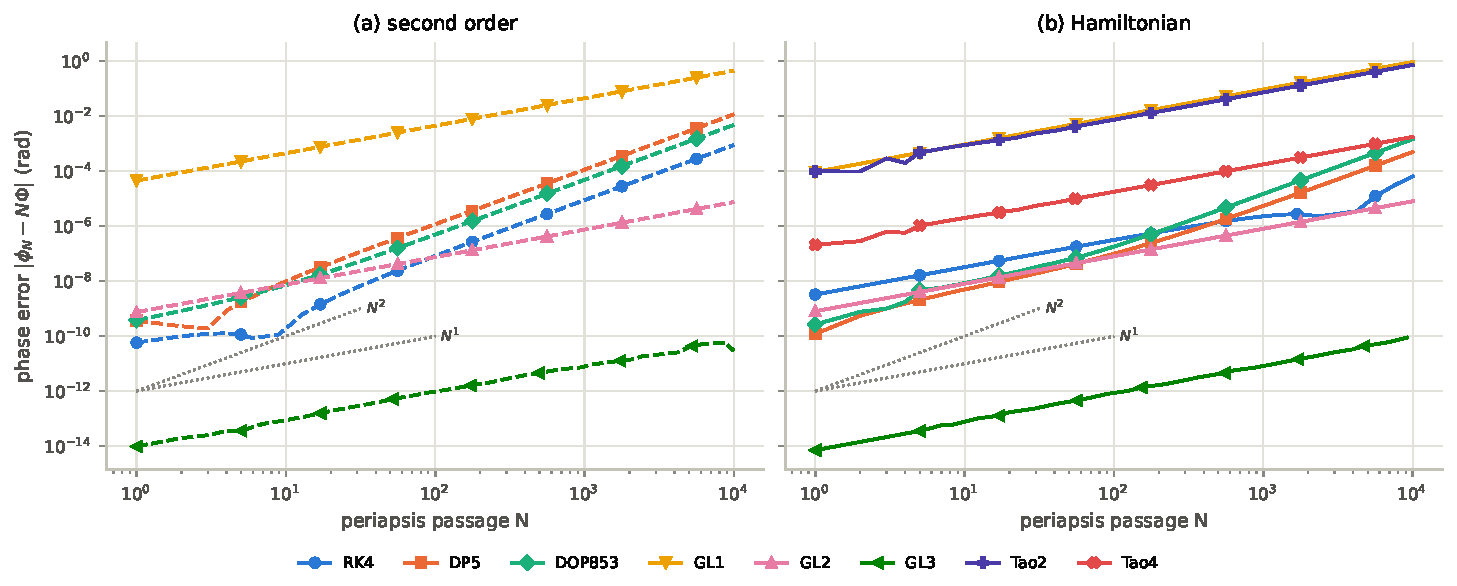
\includegraphics[width=0.95\textwidth]{F09_phase_error.pdf}
\caption{\label{fig:phase}Phase error $|\phi_N - N\Phi|$ at the $N$-th periapsis in both
formulations, with slopes 1 and 2 (F9).}
\end{figure}

\begin{table*}[t]
\caption{\label{tab:growth}Growth laws over $10^4$ periods of $(20, 0.5)$ (T4): the
mass-shell error in the last period, the log-log exponent over the last decade and its
nearest law (0, 1/2, 1, 2), the same for the phase error, and the signed fit
$\phi_N - N\Phi = c_1N + c_2N^2$ (radians per orbit and per orbit squared).}
\centering\footnotesize
% Generated by scripts/make_tables.py from results/summary/. Do not edit.
\begin{tabular}{lrrlrrlrr}
\toprule
Method & $|\delta H|$, last period & Exp. & Law & Phase error & Exp. & Law & $c_1$ & $c_2$ \\
\midrule
RK4 (b) & $1.6\times10^{-8}$ & 1.00 & linear & $6.4\times10^{-5}$ & 2.04 & quadratic & $3.2\times10^{-9}$ & $-9.6\times10^{-13}$ \\
DP5 (b) & $8.4\times10^{-8}$ & 1.00 & linear & $5.0\times10^{-4}$ & 1.97 & quadratic & $-4.9\times10^{-10}$ & $-4.9\times10^{-12}$ \\
DOP853 (b) & $2.5\times10^{-7}$ & 1.00 & linear & $1.5\times10^{-3}$ & 2.00 & quadratic & $2.4\times10^{-10}$ & $1.5\times10^{-11}$ \\
GL1 (b) & $4.0\times10^{-7}$ & 0.00 & bounded & $0.93$ & 1.00 & linear & $9.3\times10^{-5}$ & $7.5\times10^{-14}$ \\
GL2 (b) & $5.0\times10^{-12}$ & 0.00 & bounded & $8.0\times10^{-6}$ & 1.00 & linear & $8.0\times10^{-10}$ & $-2.1\times10^{-20}$ \\
GL3 (b) & $6.7\times10^{-16}$ & 0.48 & random walk & $7.3\times10^{-11}$ & 1.02 & linear & $7.0\times10^{-15}$ & $2.4\times10^{-20}$ \\
Tao2 (b) & $2.6\times10^{-6}$ & 0.00 & bounded & $0.73$ & 1.00 & linear & $-7.3\times10^{-5}$ & $1.2\times10^{-12}$ \\
Tao4 (b) & $5.2\times10^{-9}$ & 0.00 & bounded & $1.8\times10^{-3}$ & 1.00 & linear & $1.8\times10^{-7}$ & $-1.0\times10^{-15}$ \\
\midrule
RK4 (a) & $8.7\times10^{-10}$ & 0.89 & linear & $8.9\times10^{-4}$ & 2.00 & quadratic & $6.7\times10^{-11}$ & $-8.9\times10^{-12}$ \\
DP5 (a) & $2.2\times10^{-7}$ & 1.00 & linear & $0.012$ & 2.01 & quadratic & $-7.1\times10^{-9}$ & $1.2\times10^{-10}$ \\
DOP853 (a) & $9.4\times10^{-8}$ & 1.00 & linear & $4.8\times10^{-3}$ & 2.00 & quadratic & $-8.4\times10^{-11}$ & $-4.8\times10^{-11}$ \\
GL1 (a) & $4.0\times10^{-7}$ & 0.00 & bounded & $0.45$ & 1.00 & linear & $-4.5\times10^{-5}$ & $8.8\times10^{-14}$ \\
GL2 (a) & $5.0\times10^{-12}$ & 0.00 & bounded & $7.5\times10^{-6}$ & 1.00 & linear & $-7.5\times10^{-10}$ & $2.2\times10^{-18}$ \\
GL3 (a) & $3.3\times10^{-16}$ & 0.25 & random walk & $2.9\times10^{-11}$ & 0.89 & linear & $-6.8\times10^{-15}$ & $2.3\times10^{-19}$ \\
\bottomrule
\end{tabular}

\end{table*}

\paragraph{Round-off.} Compensated summation decides what happens once truncation errors are
negligible (\fig{roundoff}). On the circular orbit $r_c = 10$ every Runge--Kutta map is exact,
so the error in $\phi$ after $10^4$ orbits ($10^7$ steps) is round-off alone. With compensated
summation it is \numcircComp, 7 ulp of $\phi$. With plain summation it is \numcircPlain{} and
grows like $N^{\numcircPlainExp}$: the same increment is rounded the same way at every step,
so the errors add coherently, and each is proportional to $\phi$. GL3's mass shell follows
Brouwer's law with compensation (exponent 0.48) and grows faster without it (0.67).

\begin{figure}[t]
\centering
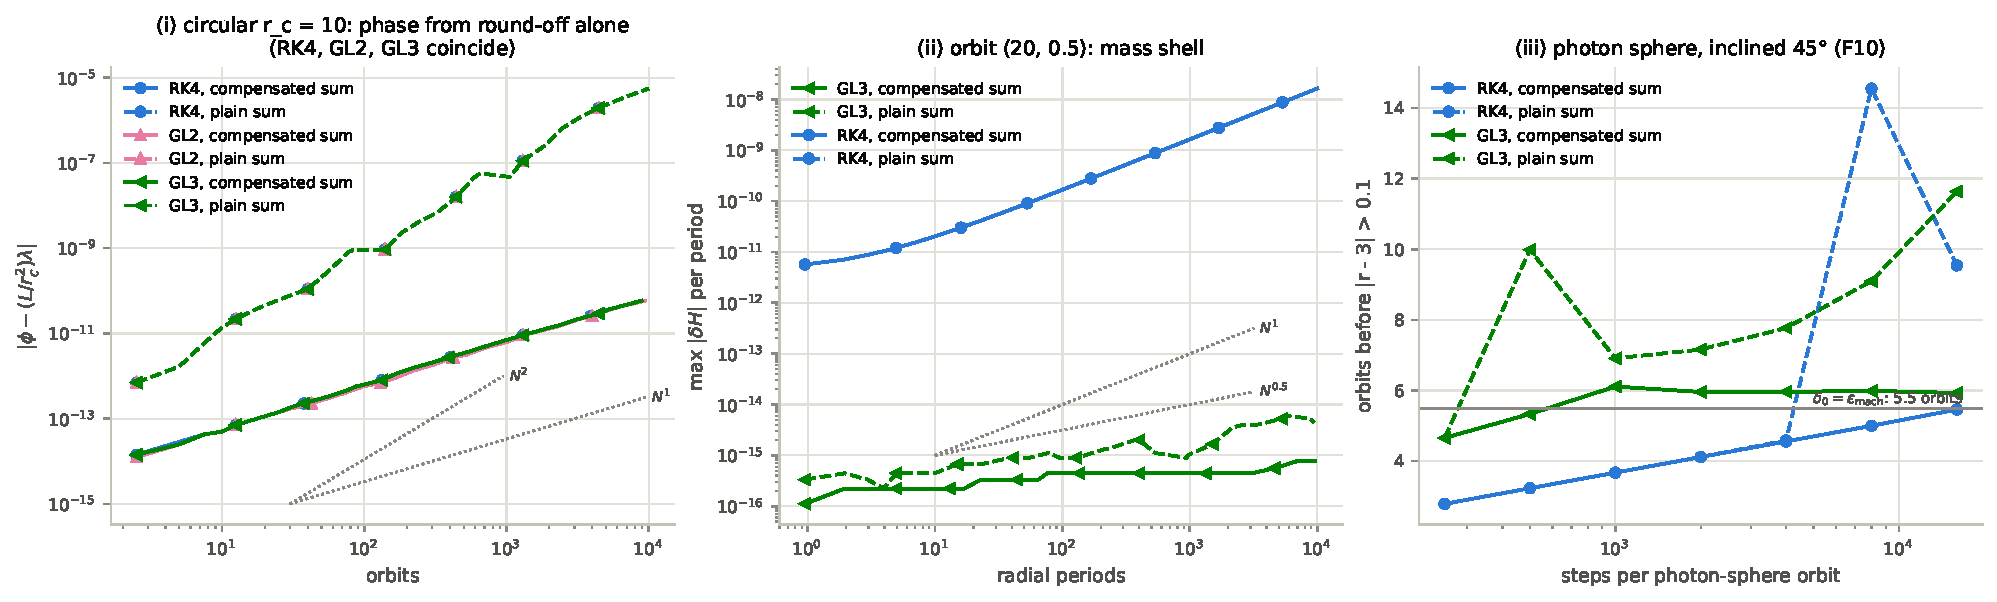
\includegraphics[width=\textwidth]{F19_roundoff.pdf}
\caption{\label{fig:roundoff}Round-off with and without compensated summation (F19). (i) Phase
of the circular orbit $r_c = 10$, where only round-off acts. (ii) Mass shell of GL3 and RK4 on
$(20, 0.5)$. (iii) Survival on the photon sphere (Sec.~\ref{sec:unstable}).}
\end{figure}

\subsection{The role of the formulation (RQ2)}
\label{sec:formulation}

In formulation (b), $E$ and $L_z$ keep their initial values bit for bit in every sample of
every method, Tao included, for all $10^4$ periods. In (a) they are nonlinear functions of the
state, and the Runge--Kutta methods drift linearly in $E$, $L_z$ and the norm, while GL1 and
GL2 stay bounded and GL3 stays at round-off (\fig{invariants}).

\begin{figure}[t]
\centering
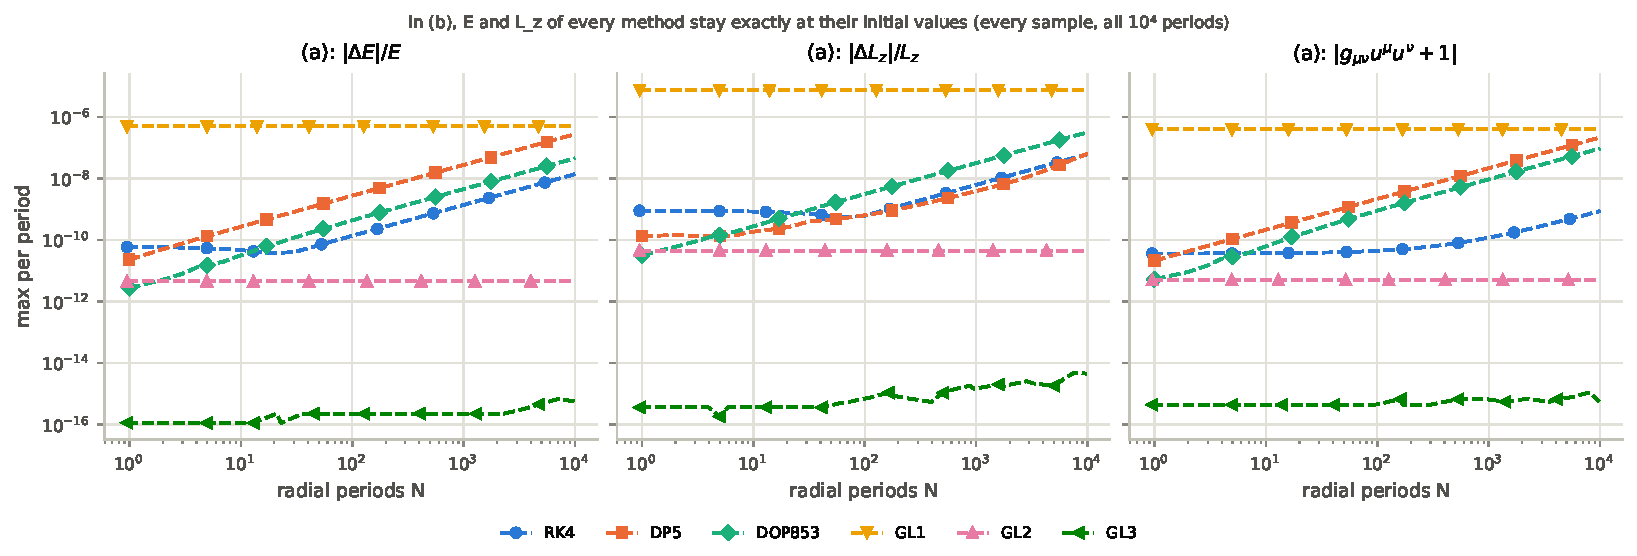
\includegraphics[width=\textwidth]{F08_invariants_formulation_a.pdf}
\caption{\label{fig:invariants}Formulation (a): relative errors in $E$, $L_z$ and the norm
over $10^4$ periods (F8). In (b), $E$ and $L_z$ do not change at all.}
\end{figure}

\textbf{Gauss--Legendre in (a), where it is symmetric but not symplectic, conserves as well as
in (b).} The largest mass-shell error of GL2 is $5.0138\times10^{-12}$ in both formulations,
equal in every printed digit, and the phase drifts are $-7.48\times10^{-10}$ and
$+8.03\times10^{-10}$ radians per orbit (\fig{symmetric}). For this integrable, reversible
system reversibility is enough, as the theory of reversible integrators
predicts~\cite[Ch.~XI]{gni2006}. RK4 drifts in both formulations.

\begin{figure}[t]
\centering
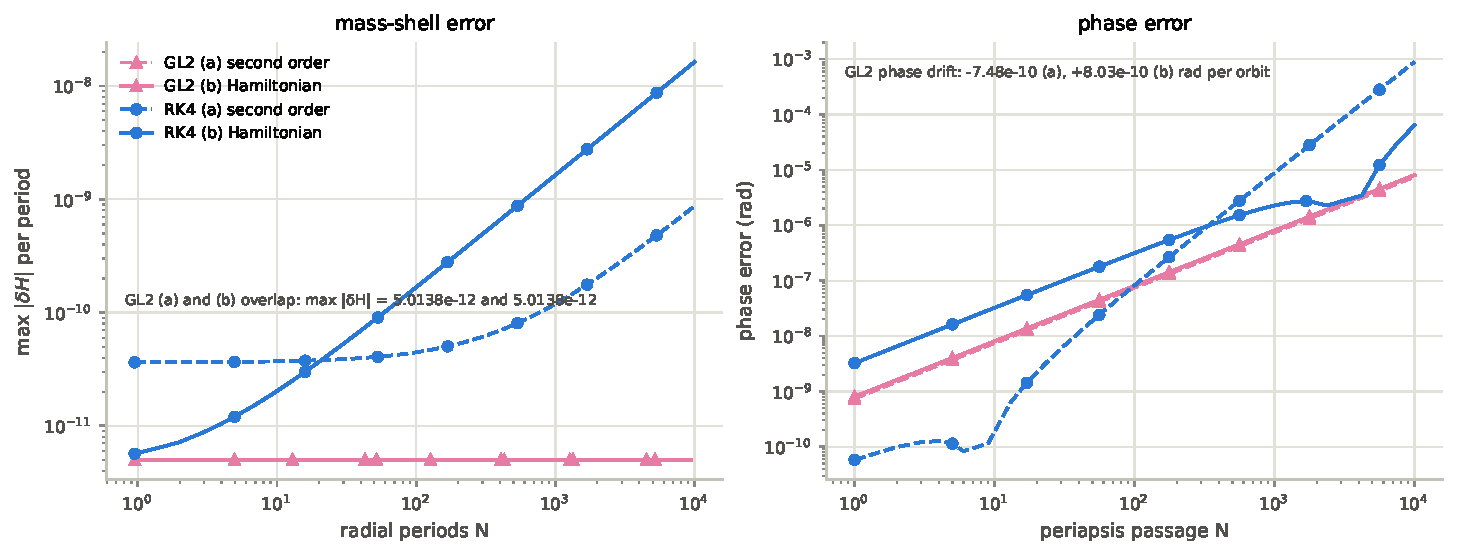
\includegraphics[width=0.95\textwidth]{F17_symmetric_vs_symplectic.pdf}
\caption{\label{fig:symmetric}GL2 in formulation (a), symmetric but not symplectic, against
GL2 in (b), symplectic, and RK4 in both (F17).}
\end{figure}

The formulation matters most for rays that travel far. In (a) the angular momentum
$L = r^2u^\phi$ is rebuilt from a component that falls like $r^{-2}$, which an absolute
tolerance cannot follow to full relative accuracy, so $L$ and with it $b = L/E$ drift. At
$b = 5.3$ and $r_\mathrm{far} = 10^4$, DOP853 at tolerance $10^{-13}$ makes an error of
$1.2\times10^{-8}$ in (a) and $3\times10^{-12}$ in (b); near $b_c$ the windings are 440 times
less accurate in (a) (\fig{windings}). At a fixed budget of $2\times10^4$ evaluations the
adaptive pairs reach $10^{-11}$--$10^{-12}$ in (b) for every $b$, but lose up to three orders
near $b_c$ in (a).

\paragraph{Inclined orbits.} $L^2$, the analogue of Carter's constant, is bounded for GL2 and
GL3 in both formulations and drifts linearly for RK4 and DOP853 (\fig{inclined}). The orbital
plane turns, and the turn is almost entirely a spurious precession of the node: the
inclination changes by at most $7\times10^{-9}$ for the Gauss methods, as it must with $L_z$
exact and $L^2$ bounded. The node precesses linearly in time for every method, symplectic or
not. Exact Schwarzschild has no nodal precession at all, so a drift in energy cannot change
the rate. Near the pole ($85^\circ$) every method is under-resolved at 1000 steps per period,
and (b) is the worse formulation: the node of GL2 drifts by $2.0\times10^{-5}$ radians per
period in (b) and $1.7\times10^{-7}$ in (a).

\begin{figure}[t]
\centering
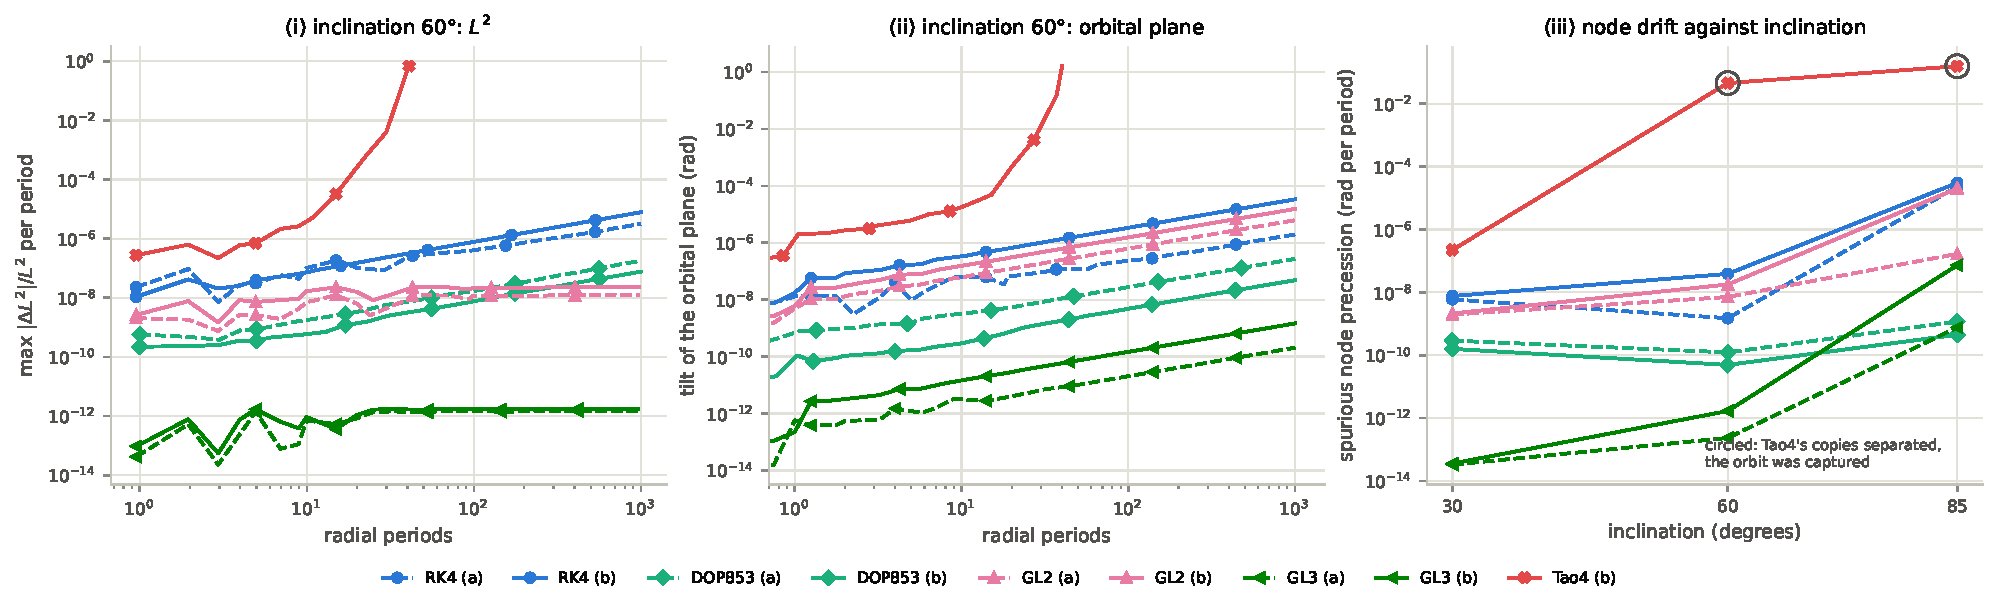
\includegraphics[width=\textwidth]{F18_inclined.pdf}
\caption{\label{fig:inclined}Inclined orbits over 1000 periods (F18): (i) $L^2$ and (ii) tilt
of the orbital plane at $60^\circ$; (iii) spurious node precession against inclination. Tao4
fails at $60^\circ$ and $85^\circ$ (Sec.~\ref{sec:method-details}).}
\end{figure}

\subsection{Long integrations: cost per accuracy (RQ3)}
\label{sec:long-cost}

\fig{long-work} repeats the work-precision comparison over 1000 periods, where errors that
grow with time have time to matter. To reach a phase error of $10^{-4}$, DOP853 is still the
cheapest method (\numlongDOPfour{} evaluations per period in (b), against
\numlongGLthreeFour{} for GL3; \tab{long-cost}). \textbf{A phase error of $10^{-8}$ is reached
by GL3 alone}, for \numlongGLthreeEight{} evaluations per period. DOP853 stops at
$4.8\times10^{-6}$ at tolerance $10^{-13}$, the tightest a double-precision controller accepts,
because its phase error grows like $N^2$. For the mass shell, $|\delta H| \le 10^{-10}$,
DOP853 remains the cheapest. Over three periods (\tab{cost}) the same orbit needed
\numshortDOP{} evaluations per period from DOP853 to reach $10^{-10}$ in phase, and
\numshortGLthree{} from GL3. The ranking turns over with the length of the integration.

\begin{figure}[t]
\centering
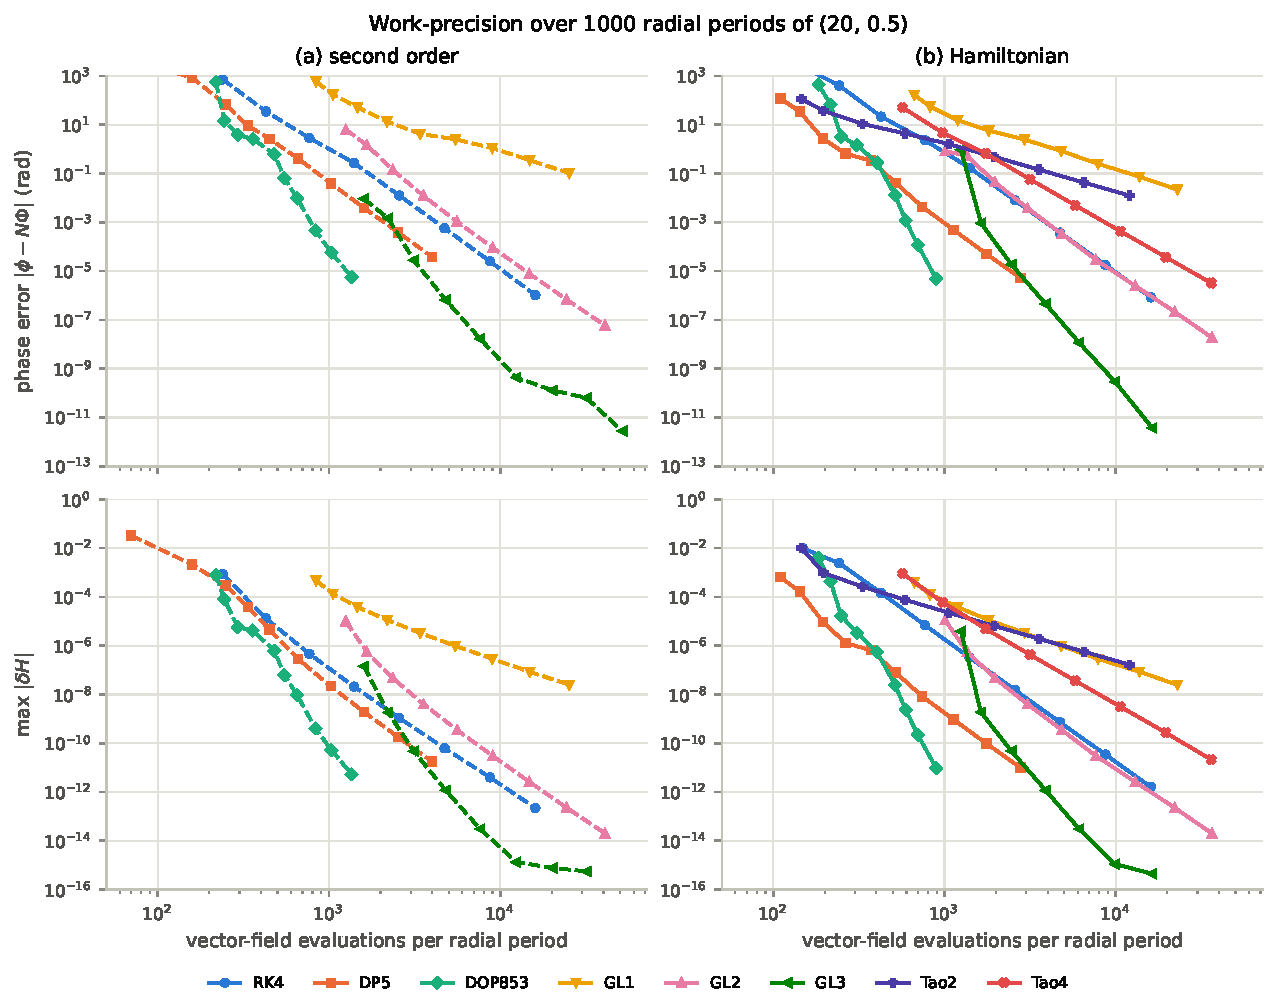
\includegraphics[width=0.9\textwidth]{F20_long_work_precision.pdf}
\caption{\label{fig:long-work}Work-precision over 1000 radial periods of $(20, 0.5)$: phase
error and largest mass-shell error against evaluations per period (F20).}
\end{figure}

\begin{table}[t]
\caption{\label{tab:long-cost}Evaluations per radial period needed over 1000 periods of
$(20, 0.5)$ (T5b), formulation (b) with (a) in parentheses.}
\centering\small
% Generated by scripts/make_tables.py from results/summary/. Do not edit.
\begin{tabular}{lrrr}
\toprule
Method & Phase $10^{-4}$ & Phase $10^{-8}$ & $|\delta H|$ $10^{-10}$ \\
\midrule
RK4 & $6.2\times10^{3}$ ($6.6\times10^{3}$) & -- & $7.0\times10^{3}$ ($4.3\times10^{3}$) \\
DP5 & $1.5\times10^{3}$ ($3.3\times10^{3}$) & -- & $1.7\times10^{3}$ ($2.8\times10^{3}$) \\
DOP853 & $706$ ($974$) & -- & $743$ ($964$) \\
GL1 & -- & -- & -- \\
GL2 & $6.1\times10^{3}$ ($8.9\times10^{3}$) & -- & $6.1\times10^{3}$ ($7.1\times10^{3}$) \\
GL3 & $2.1\times10^{3}$ ($2.8\times10^{3}$) & $6.2\times10^{3}$ ($8.2\times10^{3}$) & $2.3\times10^{3}$ ($2.9\times10^{3}$) \\
Tao2 & -- & -- & -- \\
Tao4 & $1.5\times10^{4}$ & -- & $2.5\times10^{4}$ \\
\bottomrule
\end{tabular}

\end{table}

\subsection{Unstable and marginally stable orbits (RQ4)}
\label{sec:unstable}

\paragraph{Photon sphere.} A photon starts exactly at $r = 3$ in a plane inclined by
$45^\circ$. Its only perturbation is the integration error $\delta_0$, amplified like
$e^{\lambda_L t}$ until $|r - 3| > 0.1$ after about $\ln(0.1/\delta_0)/2\pi$ orbits. If
$\delta_0$ is proportional to the tolerance, every decade of tolerance buys
$\ln 10/2\pi = 0.37$ orbits; if $\delta_0 \propto h^p$, every decade of steps buys $0.37p$.
Both predictions hold (\fig{photon}, \tab{photon}): the adaptive pairs gain 0.33--0.43 orbits
per decade (DOP853 in (b): \numpsDOPdecade); RK4, GL2 and Tao4 gain 1.38--1.49 per decade of
steps against 1.47 predicted; GL3 gains \numpsGLthreeDecade{} against 2.20. Then GL3
saturates at 5.8--6.2 orbits whatever the step. That is the round-off limit, near the
$\operatorname{arccosh}(0.1/\epsilon_\mathrm{mach})/2\pi = 5.5$ orbits of an offset of one
machine epsilon. \textbf{No method keeps a photon on the photon sphere for more than about six
orbits in double precision.} Explicit offsets $10^{-2}$--$10^{-15}$ follow the
elliptic-integral prediction to $0.01$ orbits down to $10^{-14}$.

\begin{figure}[t]
\centering
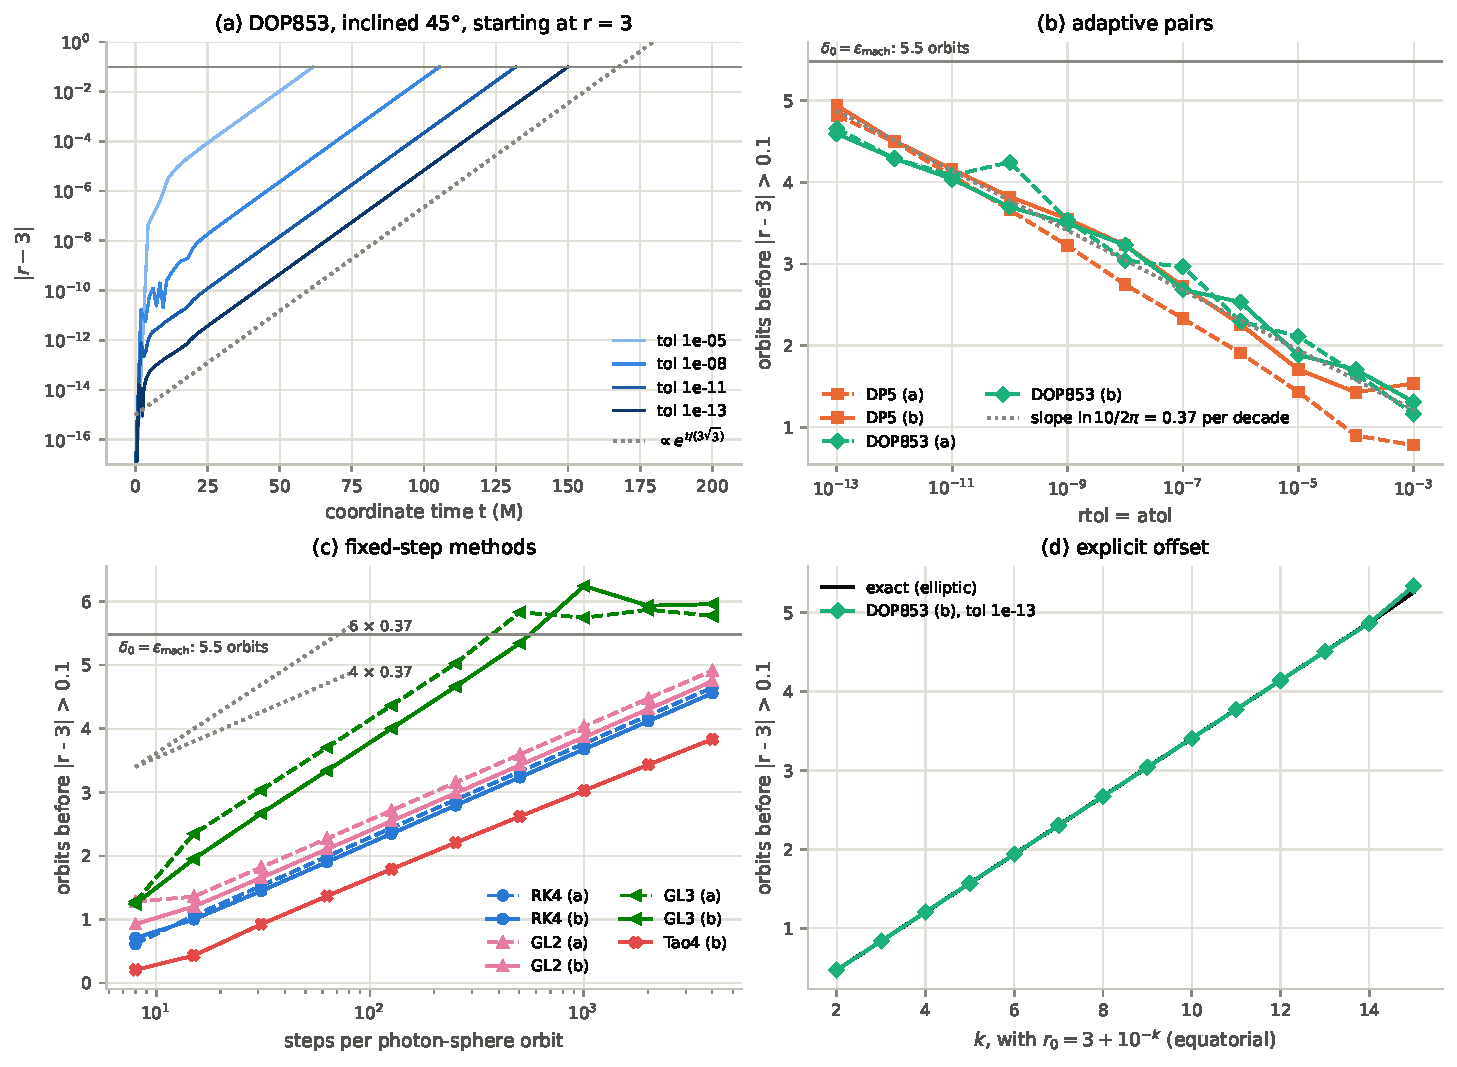
\includegraphics[width=0.95\textwidth]{F10_photon_sphere.pdf}
\caption{\label{fig:photon}Photon sphere (F10). (a) $|r - 3|$ against coordinate time for
DOP853 at four tolerances, with the growth $e^{t/3\sqrt3}$. (b), (c) Orbits survived against
tolerance and against steps per orbit. (d) Equatorial orbits from an explicit offset against
the exact prediction.}
\end{figure}

\begin{table}[t]
\caption{\label{tab:photon}Photon-sphere survival (T6): orbits gained per decade of tolerance
or of steps per orbit, against the prediction, and the orbits survived at the finest setting.}
\centering\small
% Generated by scripts/make_tables.py from results/summary/. Do not edit.
\begin{tabular}{llrrr}
\toprule
Method & Varied & Orbits per decade & Predicted & Orbits, finest \\
\midrule
DOP853 (a) & tolerance & 0.35 & 0.37 & 4.66 \\
DOP853 (b) & tolerance & 0.33 & 0.37 & 4.59 \\
DP5 (a) & tolerance & 0.43 & 0.37 & 4.82 \\
DP5 (b) & tolerance & 0.37 & 0.37 & 4.94 \\
GL2 (a) & step size & 1.41 & 1.47 & 4.91 \\
GL2 (b) & step size & 1.44 & 1.47 & 4.75 \\
GL3 (a) & step size & 2.49 & 2.20 & 5.78 \\
GL3 (b) & step size & 2.26 & 2.20 & 5.96 \\
RK4 (a) & step size & 1.49 & 1.47 & 4.65 \\
RK4 (b) & step size & 1.45 & 1.47 & 4.56 \\
Tao4 (b) & step size & 1.38 & 1.47 & 3.84 \\
\bottomrule
\end{tabular}

\end{table}

\textbf{Plain floating-point summation makes the photon sphere look more stable than it is}
(\fig{roundoff}, panel iii). With RK4 at 8000 steps per orbit the orbit survives
\numpsPlainRKfour{} orbits with plain summation, against \numpsCompRKfour{} with compensated
summation. An increment of $r$ smaller than half an ulp of 3 is lost, $r$ stays at exactly 3,
and the radial force, which is proportional to $r - 3$, stays exactly zero: rounding freezes
the instability, the longer the smaller the step. A longer survival is not always a better
integrator.

\paragraph{ISCO.} At the ISCO the effective potential has an inflection point. With
$r = 6 + \delta$ and $L^2 = 12$, $V_\mathrm{eff} = 8/9 + \delta^3/1944 + \order(\delta^4)$, and
an integration error acts as a small constant force $\varepsilon$:
\begin{equation}
  \ddot\delta = \varepsilon - \frac{\delta^2}{1296}.
  \label{eq:isco}
\end{equation}
For $\varepsilon > 0$ a stable equilibrium appears at $\delta = 36\sqrt\varepsilon$, and the
orbit oscillates about it without plunging. For $\varepsilon < 0$ it drifts inward under a
constant acceleration until $\delta \sim -36\sqrt{|\varepsilon|}$ and then runs away in a
finite time. Both stages take a time of order $|\varepsilon|^{-1/4}$. The growth is algebraic,
and the sign of the error decides whether the orbit plunges at all. With
$\varepsilon \propto h^p$ the time to plunge should scale as $n^{p/4}$ in the steps per orbit
$n$, and as $\mathrm{tol}^{-1/4}$ for the adaptive pairs. The measurements agree
(\fig{isco}): the slope is $1.11$ for RK4 in (b), $\numiscoGLtwo$ for GL2 and
$\numiscoGLthree$ for GL3 (predicted 1, 1 and 1.5), and $\numiscoDPfive$ against tolerance for
DP5 in (b). The runs that survive oscillate on the outer side, as predicted: RK4 in (a) at
100 steps per orbit stays within $6.000 < r < 6.073$ for 2000 orbits. DOP853 never plunges at
tolerances up to $10^{-6}$; DP5 in (b) plunges at $10^{-9}$--$10^{-13}$ but not at
$10^{-6}$--$10^{-8}$.

\begin{figure}[t]
\centering
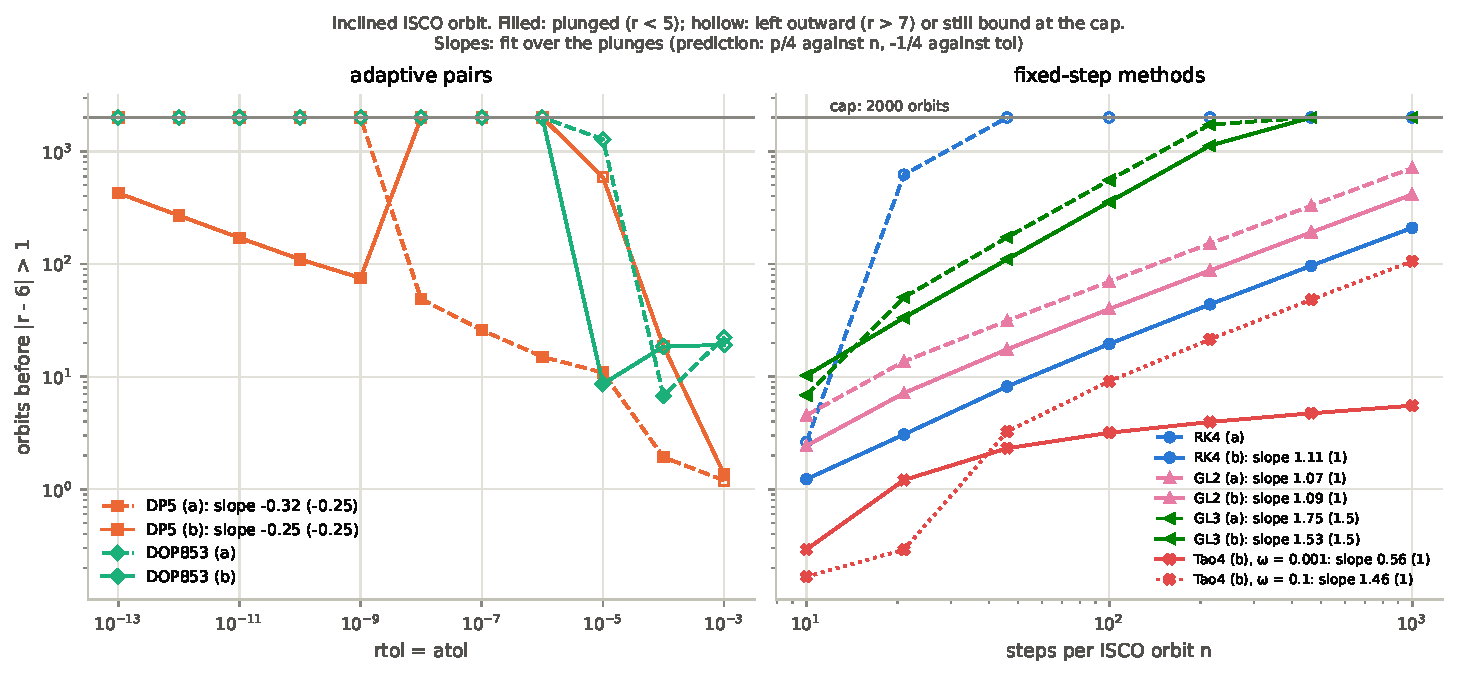
\includegraphics[width=0.95\textwidth]{F11_isco_plunge.pdf}
\caption{\label{fig:isco}Inclined ISCO orbit: orbits until $|r - 6| > 1$ against tolerance and
against steps per orbit, with the slopes fitted over the plunges (F11). Filled markers
plunged, hollow ones left outward or were still bound after 2000 orbits.}
\end{figure}

\subsection{Method-specific findings}
\label{sec:method-details}

\paragraph{Tao's coupling $\omega$.} The error of Tao4 grows in proportion to $\omega$ once
$\omega h \gtrsim 10^{-3}$, and the method diverges for $\omega h \gtrsim 1.4$; too small an
$\omega$ lets the copies separate, by up to 23 within 300 periods for $\omega = 10^{-5}$
(\fig{tao}). We use $\omega = 10^{-3}$ throughout: within a factor 1.2--5 of the best value
on the orbits tested, with the copies within $3\times10^{-6}$ over 300 periods. This choice
fails on two of the long experiments. On the ISCO the copies separate by $1.7$ in $r$ and the orbit
plunges within six orbits whatever the step; $\omega = 0.1$ holds them together. On the
inclined orbits the run is captured after 41 periods at $60^\circ$ and after 3 at $85^\circ$;
a larger $\omega$ helps at $60^\circ$ but leaves $L^2$ drifting 3000 times more than with
GL2, and no $\omega$ between $10^{-3}$ and 1 works at $85^\circ$. The coupling is a
problem-dependent parameter, and choosing it is a real cost of the method.

\paragraph{Implicit iteration.} Iterations per step grow from 2--5 at small steps to 10--23 at
the largest; GL3 needs the fewest, and (a) needs more than (b) (\fig{implicit}). Stopping the
iteration at a tolerance instead of at stagnation makes GL2 drift: over 1000 periods $|\delta
H|$ grows tenfold with tolerances $10^{-6}$ and $10^{-8}$, threefold with $10^{-10}$, and not
at all with $10^{-12}$ or at stagnation. A tolerance of $10^{-12}$ needs 3.5 iterations per
step against 6.7 for stagnation: the round-off rule is safe but not the cheapest safe rule.

\paragraph{Adaptive steps.} On the deflection the step grows roughly in proportion to $r$, and
DOP853 needs three to four times fewer steps than DP5 at the same tolerance (\fig{steps}).

\begin{figure}[t]
\centering
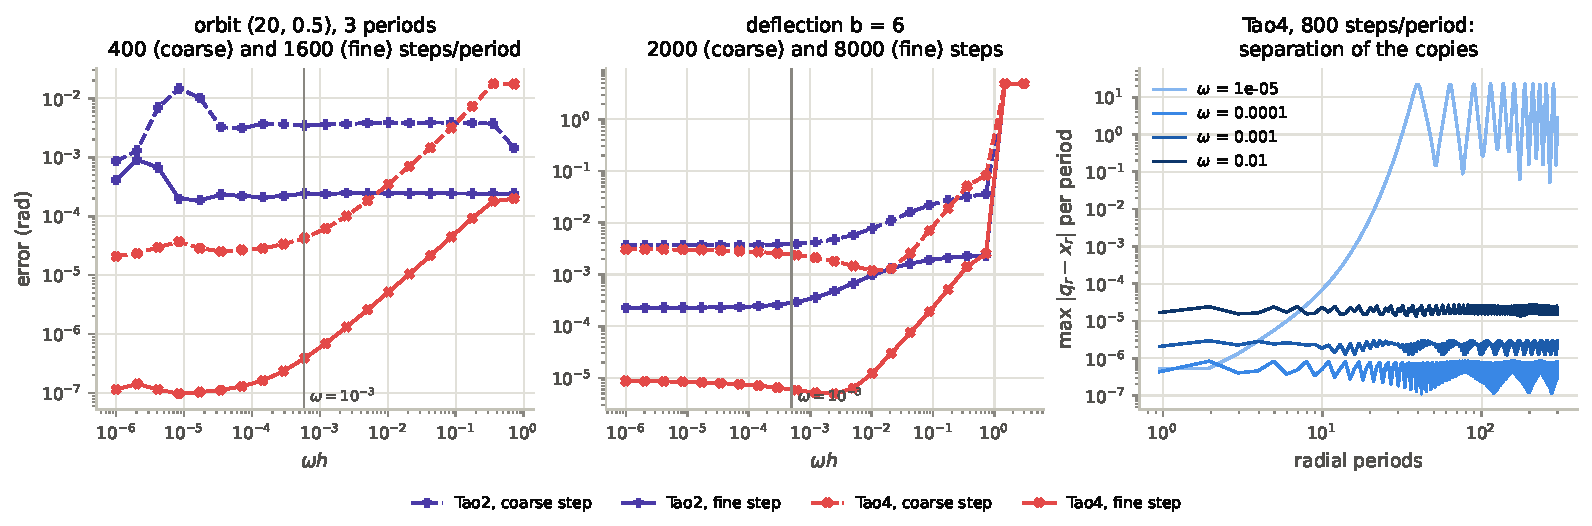
\includegraphics[width=0.75\textwidth]{F14_tao_omega.pdf}
\caption{\label{fig:tao}Tao4: error against the coupling $\omega$ at fixed step, and the
separation of the two copies (F14).}
\end{figure}

\begin{figure}[t]
\centering
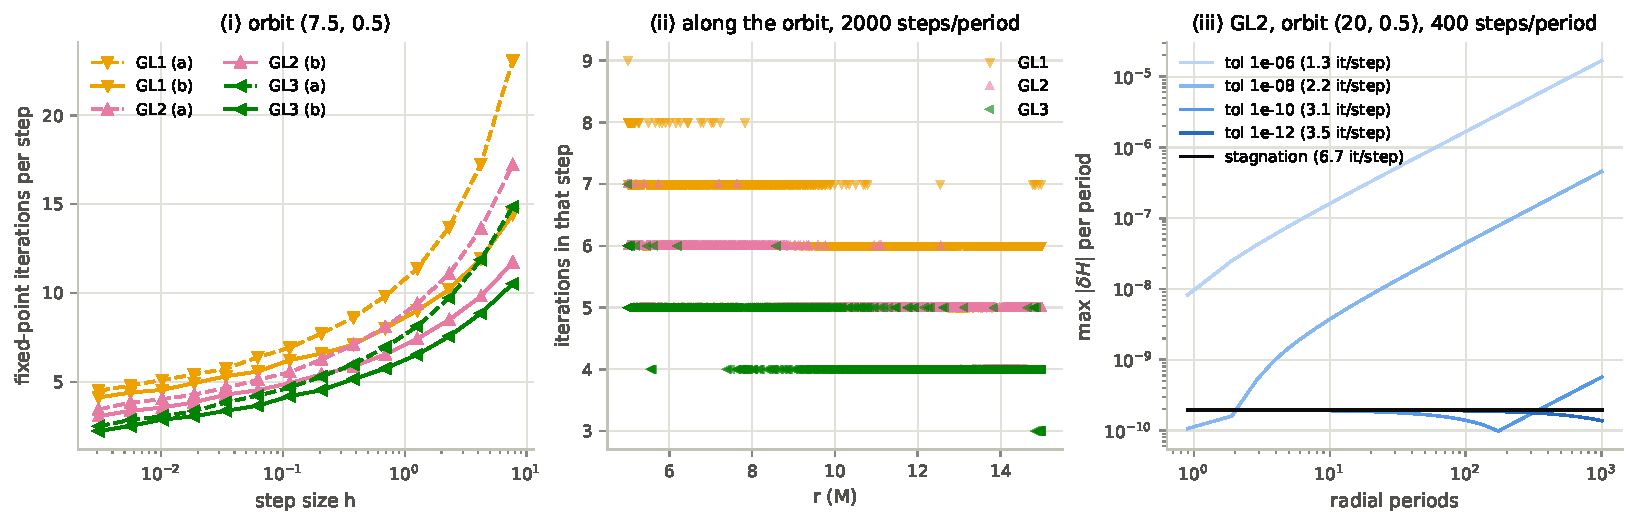
\includegraphics[width=\textwidth]{F15_implicit.pdf}
\caption{\label{fig:implicit}Gauss--Legendre iteration (F15): iterations per step against $h$
and along the orbit, and the drift of $|\delta H|$ when the iteration stops at a tolerance.}
\end{figure}

\begin{figure}[t]
\centering
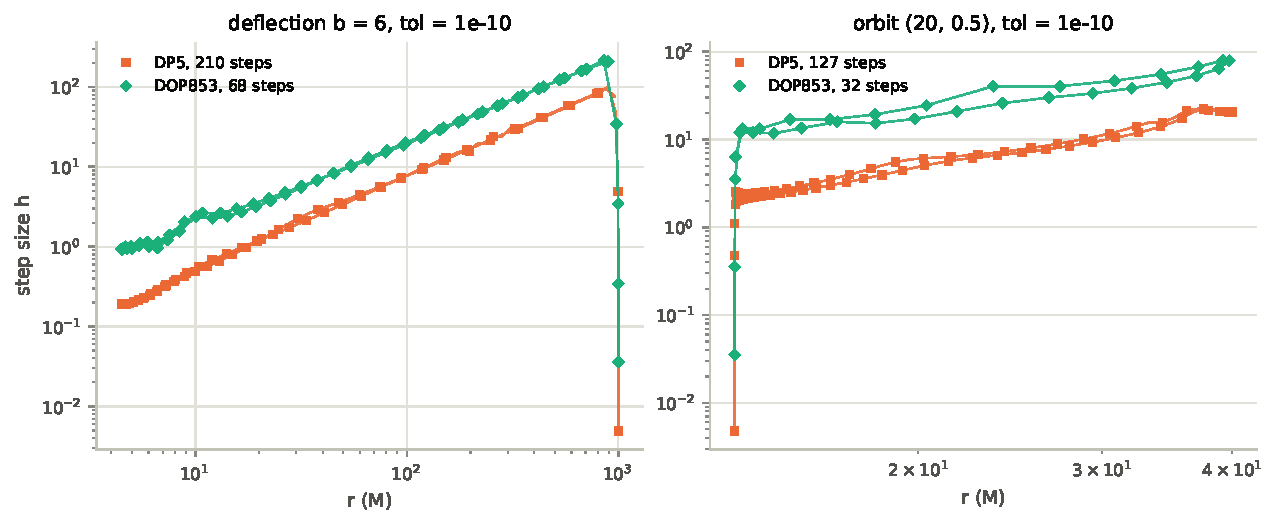
\includegraphics[width=0.75\textwidth]{F16_step_history.pdf}
\caption{\label{fig:steps}Step sizes of the adaptive pairs against $r$ on the deflection and
on an eccentric orbit (F16).}
\end{figure}

\section{Discussion and recommendations}
\label{sec:discussion}

\paragraph{Answers to the research questions.}
\RQ{1}: the Runge--Kutta methods, fixed-step or adaptive, drift linearly in the mass shell and
quadratically in phase. The symplectic methods keep the mass-shell error bounded at
$\order(h^p)$ and the phase error linear, and once their truncation error falls below
round-off, compensated summation gives Brouwer's $N^{1/2}$.
\RQ{2}: in Hamilton's form $E$ and $L_z$ are exact for every method; in the second-order form
they drift for every non-geometric method. Formulation (b) is up to 440 times more accurate
for rays that go far out. Symmetry alone gives Gauss--Legendre in (a) the same bounded errors
as in (b). The one case that favours (a) is the near-polar orbit, where the spurious node
precession is about 100 times smaller.
\RQ{3}: DOP853 is the cheapest method over a few periods at every accuracy and over 1000
periods for modest accuracy; for a phase error of $10^{-8}$ over 1000 periods only GL3
delivers. Tao4 is never competitive.
\RQ{4}: on the photon sphere accuracy buys survival logarithmically, $\ln 10/2\pi$ orbits per
decade, up to about six orbits in double precision for every method. At the ISCO the time to
plunge grows algebraically, as $|\varepsilon|^{-1/4}$, and an error of the stabilizing sign
prevents the plunge.

\begin{table*}[t]
\caption{\label{tab:recommendations}Recommendations (T7), with the evidence they rest on.}
\centering\small
\begin{tabular}{>{\raggedright\arraybackslash}p{0.24\textwidth}>{\raggedright\arraybackslash}p{0.30\textwidth}>{\raggedright\arraybackslash}p{0.38\textwidth}}
\toprule
Task & Recommendation & Evidence \\
\midrule
Ray tracing, short integrations (deflection, a few orbits)
  & DOP853 in formulation (b)
  & Cheapest at every accuracy (\tab{cost}); exact $E$, $L_z$ and up to 440 times more
    accurate than (a) near $b_c$ (\fig{windings}). \\ \addlinespace
Long orbit evolution where the phase matters ($10^3$ periods and more)
  & GL3 in (b), iterated to stagnation (or to $10^{-12}$), with compensated summation
  & The only method to reach a phase error of $10^{-8}$ over 1000 periods (\tab{long-cost});
    bounded invariants (\fig{energy}); Brouwer's law (\fig{roundoff}). \\ \addlinespace
Long runs at modest accuracy
  & DOP853 is cheaper, but its invariants drift linearly
  & \tab{long-cost}, \fig{energy}, \fig{phase}. \\ \addlinespace
Studies that need bounded invariants (Poincar\'e sections, statistics of chaotic orbits)
  & A Gauss method with fixed step, in either formulation
  & Bounded $H$, $L^2$ in (a) and (b) (\fig{symmetric}, \fig{inclined}). \\ \addlinespace
Unstable orbits (photon sphere)
  & Any accurate method with compensated summation; expect at most $\sim$6 orbits
  & \fig{photon}, \tab{photon}; plain summation fakes survival (\fig{roundoff}). \\ \addlinespace
Explicit symplectic integration of a general metric
  & Tao's method only with $\omega$ tuned for the problem at hand
  & Fails on the ISCO and on inclined orbits with $\omega$ tuned on a stable orbit
    (Sec.~\ref{sec:method-details}). \\
\bottomrule
\end{tabular}
\end{table*}

\paragraph{Recommendations.} \tab{recommendations} turns these answers into advice (\RQ{5}).
Two conclusions go beyond the hypotheses we started from. First, the cost advantage of the
adaptive pair is large enough that geometric integration pays off only when the integration
is long \emph{and} the phase matters. Over $10^3$ periods a mass-shell error of $10^{-10}$
is cheaper to buy with a tight tolerance than with a symplectic method, although the drift
of DOP853 will overtake the bounded error of GL3 on longer runs. Second, the round-off details matter: compensated
summation turns a quadratic phase drift into a few ulp, and its absence can make an
integration look more stable than the physics allows.

\paragraph{Limitations.} The study uses fixed steps for the geometric methods; variable steps
destroy their long-time properties unless the time is transformed~\cite{calvo1993,gni2006},
and Ref.~\cite{seyrich2012} shows one way to combine them. Only Schwarzschild is covered,
where $t$ and $\phi$ are cyclic and the problem is integrable; in nonintegrable systems
(charged or spinning particles, perturbed metrics) the advantage of symplectic methods should
be larger. Wall times compare our own implementations, whose generic step code costs 2--5
times the bare vector field, so they are not a statement about the algorithms' intrinsic
cost. The explicit symplectic splittings of Wang et al.~\cite{wang2021} and Taylor
methods~\cite{biscani2021} were not tested.

\paragraph{Extension to Kerr.} The metric interface takes the full inverse metric and its
derivatives, and none of the integrators or formulations knows the metric. Adding Kerr in
Boyer--Lindquist coordinates is a new metric class, analytic references (Carter's constant,
spherical photon orbits) and new test cases, with no change to the integrator code. The
inclined orbits of TC6 already exercise the code path that will monitor Carter's constant.

\section{Conclusions}
\label{sec:conclusions}

We compared eight integrators on Schwarzschild geodesics in two formulations, against exact
references, over integrations from a single deflection to $10^4$ orbits. The classical
expectations of geometric integration hold quantitatively: linear against quadratic phase
error, linear drift against bounded invariants, Brouwer's law at round-off, and symmetric
methods behaving like symplectic ones on this reversible, integrable system. The practical
picture is less one-sided than the theory suggests. A high-order adaptive Runge--Kutta pair is
the right tool for ray tracing and for long runs at modest accuracy. Sixth-order
Gauss--Legendre is the right tool when the phase must stay accurate over thousands of orbits.
Tao's explicit symplectic method needs a coupling tuned to each problem.

Two results concern orbits at the edge of stability. On the photon sphere, accuracy buys
survival only logarithmically, and double precision caps it at about six orbits for every
method. At the ISCO the integration error decides, through its sign, whether an orbit plunges
at all, and through its size, as $|\varepsilon|^{-1/4}$, when. In both cases the rounding of
the state update, compensated or not, changes the answer qualitatively.

All code, cached summaries, figures and this report are produced by \texttt{make all} from a
clean checkout. The interface between metric and integrator is ready for the Kerr metric, the
next step of this work, and for its (anti-)de~Sitter generalizations.


\begin{acknowledgments}
The numerical work uses NumPy~\cite{numpy}, SciPy~\cite{scipy}, Numba~\cite{numba},
mpmath~\cite{mpmath} and Matplotlib~\cite{matplotlib}. Code, data and the scripts that produce
every figure and table are available at \repo.
\end{acknowledgments}

\appendix
\section{Christoffel symbols and Hamilton's equations}
\label{app:christoffel}

The nine independent non-zero Christoffel symbols of the Schwarzschild metric are
\begin{gather*}
\Gamma^t_{tr} = \frac{1}{r(r - 2)}, \qquad
\Gamma^r_{tt} = \frac{r - 2}{r^3}, \qquad
\Gamma^r_{rr} = -\frac{1}{r(r - 2)}, \qquad
\Gamma^r_{\theta\theta} = -(r - 2), \\
\Gamma^r_{\phi\phi} = -(r - 2)\sin^2\theta, \qquad
\Gamma^\theta_{r\theta} = \Gamma^\phi_{r\phi} = \frac1r, \qquad
\Gamma^\theta_{\phi\phi} = -\sin\theta\cos\theta, \qquad
\Gamma^\phi_{\theta\phi} = \cot\theta .
\end{gather*}
The code writes them in terms of $r - 2$ rather than $f = 1 - 2/r$, which keeps every
component accurate to full relative precision down to the horizon. Hamilton's equations for
(\ref{eq:hamiltonian}) are
\begin{gather*}
\dot t = -\frac{p_t}{f}, \quad \dot r = f p_r, \quad \dot\theta = \frac{p_\theta}{r^2}, \quad
\dot\phi = \frac{p_\phi}{r^2\sin^2\theta}, \qquad \dot p_t = \dot p_\phi = 0, \\
\dot p_r = -\frac{f'}{2}\left(\frac{p_t^2}{f^2} + p_r^2\right)
  + \frac{1}{r^3}\left(p_\theta^2 + \frac{p_\phi^2}{\sin^2\theta}\right), \qquad
\dot p_\theta = \frac{\cos\theta}{r^2\sin^3\theta}\,p_\phi^2 .
\end{gather*}
Both sets were checked against a symbolic derivation from $g_{\mu\nu}$ evaluated at 50 digits,
to $6\times10^{-16}$ relative per component for $r - 2$ from $10^{-8}$ to $10^4$.

\section{Gauss--Legendre methods}
\label{app:gauss}

The $s$-stage Gauss method has nodes $c_i$ at the zeros of the shifted Legendre polynomial of
degree $s$, and $a_{ij} = \int_0^{c_i}\ell_j(\tau)\,\dd\tau$, $b_j = \int_0^1\ell_j(\tau)\,\dd\tau$
with the Lagrange polynomials $\ell_j$ on the nodes. For $s = 2$,
\begin{equation*}
\begin{array}{c|cc}
\tfrac12 - \tfrac{\sqrt3}{6} & \tfrac14 & \tfrac14 - \tfrac{\sqrt3}{6} \\[2pt]
\tfrac12 + \tfrac{\sqrt3}{6} & \tfrac14 + \tfrac{\sqrt3}{6} & \tfrac14 \\[2pt]
\hline
 & \tfrac12 & \tfrac12
\end{array}
\qquad\text{and for } s = 3,\qquad
\begin{array}{c|ccc}
\tfrac12 - \tfrac{\sqrt{15}}{10} & \tfrac{5}{36} & \tfrac29 - \tfrac{\sqrt{15}}{15} & \tfrac{5}{36} - \tfrac{\sqrt{15}}{30} \\[2pt]
\tfrac12 & \tfrac{5}{36} + \tfrac{\sqrt{15}}{24} & \tfrac29 & \tfrac{5}{36} - \tfrac{\sqrt{15}}{24} \\[2pt]
\tfrac12 + \tfrac{\sqrt{15}}{10} & \tfrac{5}{36} + \tfrac{\sqrt{15}}{30} & \tfrac29 + \tfrac{\sqrt{15}}{15} & \tfrac{5}{36} \\[2pt]
\hline
 & \tfrac{5}{18} & \tfrac49 & \tfrac{5}{18}
\end{array}
\end{equation*}
GL1 is the implicit midpoint rule ($c = a = \tfrac12$, $b = 1$). One step solves
$Z_i = h\sum_j a_{ij}F(y_n + Z_j)$ by fixed-point iteration and sets
$y_{n+1} = y_n + \sum_i d_i Z_i$ with $d^\mathsf{T} = b^\mathsf{T}A^{-1}$, which avoids a final
evaluation of $F$. The start value of $Z$ is the collocation polynomial of the previous step,
evaluated at the new nodes. The iteration stops when $\|\Delta Z\|$ no longer decreases and is
within 100 ulp of $\|Z\|$ (Sec.~\ref{sec:integrators}), or after 60 iterations, which never
occurred in the experiments.

\section{Reproducibility and computing environment}
\label{app:environment}

All integrators, metrics and formulations are compiled with Numba~\cite{numba}. One compiled
driver per kind of method receives the vector field as a typed first-class function, so that
compilation happens once per machine (about 60~s) and is cached. Every run is described by a
specification (test case, formulation, method, options) whose hash keys a cache of result rows
that carry the git commit, library versions and CPU. Long runs are reduced to per-period
maxima before caching. The command \texttt{make all} regenerates every figure and table from
an empty cache and then compiles this report; on the machine of \tab{environment} it takes
about 23 minutes on four cores. Repeating it reproduced every summary table and figure byte
for byte, except the wall times, which agreed to within 25\% (median ratio 0.98).

\begin{table}[h]
\caption{\label{tab:environment}Computing environment of the results (T8).}
\centering\small
% Generated by scripts/make_tables.py from results/summary/. Do not edit.
\begin{tabular}{ll}
\toprule
Item & Value \\
\midrule
CPU & Intel(R) Core(TM) i5-7300HQ CPU @ 2.50GHz \\
logical cores & 4 \\
operating system & Linux-7.0.0-34-generic-x86\_64-with-glibc2.43 \\
Python & 3.14.7 \\
numpy & 2.5.3 \\
scipy & 1.18.1 \\
numba & 0.68.0 \\
llvmlite & 0.50.0 \\
mpmath & 1.3.0 \\
matplotlib & 3.11.2 \\
pandas & 3.0.6 \\
geoint & 1.0.0 \\
threads per process & 1 (NUMBA\_NUM\_THREADS = OMP\_NUM\_THREADS = 1) \\
parallel sweeps & up to 4 forked worker processes; timing runs one at a time \\
timing & median of 2 repeats after a warm-up run (ADR 0003) \\
floating point & IEEE 754 double; compensated summation in fixed-step updates \\
\bottomrule
\end{tabular}

\end{table}


\bibliography{refs}

\end{document}
